% -----------------------------------------------------------
%
%  CHAPTER 6  of Quantum information with atoms and photons
%
%  written by Francesco Barone, Jan 2023
%  contributions from Giosuè Sardo Infirri
% -----------------------------------------------------------


Different strategies are used to correlate energy levels of a system made of more than one atom.\\

\noindent \textbf{\sffamily Rydberg strategy}\\

The Rydberg atoms technology is based on the fact that there are infinite energy levels before the ionization of an atom. A \textit{Rydberg atom} is an excited atom with one or more electrons that have a very high principal quantum number $n$.
\\
Some properties of the Rydberg atoms are good response to electric and magnetic fields, long decay periods and electron wavefunctions that approximate, under some conditions, classical orbits of electrons around the nucleus.
\\
Since the radius of the orbit scales as $n^{2}$ and the geometric cross-section as $n^{4}$, these atoms that are extremely large, with loosely bounded valence electrons, are easily perturbed or ionized by collisions and external fields. In particular, we are able to ionize atoms up to the levels $50\,S-100\,S$, where they have a radius of the order of 1 $\mu$m ($10^{4}$ times larger than that of an atom in ground state). 
\\
Such properties permit to interact and manipulate these atoms efficiently. \\

\noindent\textbf{\sffamily Ion traps}\\

Another strategy consists of trapping many similar ions in an harmonic potential, like a sort of lattice\footnote{We (students) suggest to look at this documentation (\href{https://pennylane.ai/qml/demos/tutorial_trapped_ions.html}{Pennylane: Trapped ion quantum computers}) for a very general overview of trapped ion quantum computers.}. The Coulomb interaction between the centre of mass of the ions is relevant and two types of degrees of freedom are present: 
\begin{itemize}
    \setlength\itemsep{1em}
    \item external degrees of freedom, which correspond to the center of mass position; 
    \item internal degrees of freedom, which correspond to the electronic levels. 
\end{itemize}
It is important to notice that the interaction between the external degrees of freedom of different atoms is always established, while the one between the internal and the external ones is more complicated and it is discussed in the following section. 

\section{Lamb-Dicke coupling for a trapped ion}
Consider a system made of: 
\begin{itemize}
    \item an hydrogen-like atom;
    \item an harmonic trap for the centre-of-mass coordinate; 
    \item a laser with a frequency close to one associated to an optical transition.
\end{itemize}

\begin{center}


\tikzset{every picture/.style={line width=0.75pt}} %set default line width to 0.75pt        

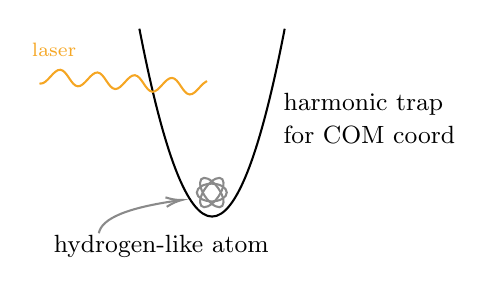
\begin{tikzpicture}[x=0.75pt,y=0.75pt,yscale=-1,xscale=1]
%uncomment if require: \path (0,126); %set diagram left start at 0, and has height of 126

%Shape: Parabola [id:dp6726865290868447] 
\draw   (57.33,1.49) .. controls (80.67,122.17) and (104,122.17) .. (127.33,1.49) ;
%Shape: Wave [id:dp7512032357045172] 
\draw  [color={rgb, 255:red, 245; green, 166; blue, 35 }  ,draw opacity=1 ] (9.18,27.82) .. controls (9.35,27.88) and (9.53,27.91) .. (9.71,27.93) .. controls (11.34,28.05) and (12.87,26.36) .. (14.47,24.6) .. controls (16.07,22.83) and (17.6,21.15) .. (19.22,21.27) .. controls (20.85,21.39) and (22.12,23.27) .. (23.44,25.25) .. controls (24.77,27.23) and (26.04,29.12) .. (27.66,29.24) .. controls (29.29,29.36) and (30.82,27.67) .. (32.42,25.91) .. controls (34.02,24.14) and (35.55,22.46) .. (37.17,22.58) .. controls (38.8,22.7) and (40.07,24.58) .. (41.39,26.56) .. controls (42.72,28.54) and (43.99,30.43) .. (45.62,30.55) .. controls (47.24,30.66) and (48.77,28.98) .. (50.37,27.22) .. controls (51.97,25.45) and (53.5,23.77) .. (55.13,23.89) .. controls (56.75,24) and (58.02,25.89) .. (59.35,27.87) .. controls (60.67,29.85) and (61.94,31.74) .. (63.57,31.85) .. controls (65.19,31.97) and (66.72,30.29) .. (68.32,28.52) .. controls (69.92,26.76) and (71.45,25.08) .. (73.08,25.19) .. controls (74.7,25.31) and (75.97,27.2) .. (77.3,29.18) .. controls (78.63,31.16) and (79.9,33.04) .. (81.52,33.16) .. controls (83.15,33.28) and (84.68,31.6) .. (86.28,29.83) .. controls (87.5,28.48) and (88.68,27.18) .. (89.9,26.7) ;
%Shape: Ellipse [id:dp06930515818625183] 
\draw  [color={rgb, 255:red, 138; green, 138; blue, 138 }  ,draw opacity=1 ] (85,80.41) .. controls (85,78.06) and (88.23,76.15) .. (92.21,76.15) .. controls (96.19,76.15) and (99.42,78.06) .. (99.42,80.41) .. controls (99.42,82.77) and (96.19,84.68) .. (92.21,84.68) .. controls (88.23,84.68) and (85,82.77) .. (85,80.41) -- cycle ;
%Shape: Ellipse [id:dp5001538841210537] 
\draw  [color={rgb, 255:red, 138; green, 138; blue, 138 }  ,draw opacity=1 ] (87.11,74.02) .. controls (88.44,72.35) and (91.8,73.87) .. (94.61,77.4) .. controls (97.43,80.93) and (98.64,85.15) .. (97.31,86.81) .. controls (95.98,88.48) and (92.63,86.96) .. (89.81,83.43) .. controls (86.99,79.89) and (85.79,75.68) .. (87.11,74.02) -- cycle ;
%Shape: Ellipse [id:dp5281934647928739] 
\draw  [color={rgb, 255:red, 138; green, 138; blue, 138 }  ,draw opacity=1 ] (87.11,86.81) .. controls (85.79,85.15) and (86.99,80.93) .. (89.81,77.4) .. controls (92.63,73.87) and (95.98,72.35) .. (97.31,74.02) .. controls (98.64,75.68) and (97.43,79.89) .. (94.61,83.43) .. controls (91.8,86.96) and (88.44,88.48) .. (87.11,86.81) -- cycle ;
%Curve Lines [id:da8270564180244198] 
\draw [color={rgb, 255:red, 138; green, 138; blue, 138 }  ,draw opacity=1 ]   (37.78,100.02) .. controls (39.06,93) and (51.13,87.76) .. (75.85,84.28) ;
\draw [shift={(77.78,84.02)}, rotate = 172.4] [color={rgb, 255:red, 138; green, 138; blue, 138 }  ,draw opacity=1 ][line width=0.75]    (7.65,-2.3) .. controls (4.86,-0.97) and (2.31,-0.21) .. (0,0) .. controls (2.31,0.21) and (4.86,0.98) .. (7.65,2.3)   ;

% Text Node
\draw (4,7) node [anchor=north west][inner sep=0.75pt]  [font=\scriptsize,color={rgb, 255:red, 245; green, 166; blue, 35 }  ,opacity=1 ] [align=left] {laser};
% Text Node
\draw (125.33,31) node [anchor=north west][inner sep=0.75pt]   [align=left] {{\small harmonic trap}\\{\small for COM coord}};
% Text Node
\draw (14.67,99.67) node [anchor=north west][inner sep=0.75pt]   [align=left] {{\small hydrogen-like atom}};


\end{tikzpicture}

\end{center}


\begin{tcolorbox} [breakable, enhanced]
\textbf{Example: Ca$^+$ ion} \\
A $Ca^+$ ion resembles very much an hydrogen-like atom, with $Z_{\text{eff}}=2$
\begin{center}


\tikzset{every picture/.style={line width=0.75pt}} %set default line width to 0.75pt        

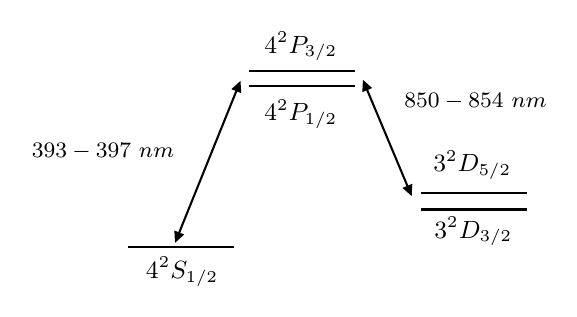
\begin{tikzpicture}[x=0.75pt,y=0.75pt,yscale=-1,xscale=1]
%uncomment if require: \path (0,143); %set diagram left start at 0, and has height of 143

%Straight Lines [id:da5956637591220642] 
\draw    (114.5,35.63) -- (165.47,35.63) ;
%Straight Lines [id:da2361976767409908] 
\draw    (56.5,113) -- (107.47,113) ;
%Straight Lines [id:da28949153423771146] 
\draw    (197.5,95) -- (248.47,95) ;
%Straight Lines [id:da7754664280521243] 
\draw    (109.39,35.82) -- (80.14,108.26) ;
\draw [shift={(79.02,111.04)}, rotate = 291.99] [fill={rgb, 255:red, 0; green, 0; blue, 0 }  ][line width=0.08]  [draw opacity=0] (5.36,-2.57) -- (0,0) -- (5.36,2.57) -- cycle    ;
\draw [shift={(110.52,33.04)}, rotate = 111.99] [fill={rgb, 255:red, 0; green, 0; blue, 0 }  ][line width=0.08]  [draw opacity=0] (5.36,-2.57) -- (0,0) -- (5.36,2.57) -- cycle    ;
%Straight Lines [id:da4862607788094553] 
\draw    (170.68,35.31) -- (191.86,85.78) ;
\draw [shift={(193.02,88.54)}, rotate = 247.23] [fill={rgb, 255:red, 0; green, 0; blue, 0 }  ][line width=0.08]  [draw opacity=0] (5.36,-2.57) -- (0,0) -- (5.36,2.57) -- cycle    ;
\draw [shift={(169.52,32.54)}, rotate = 67.23] [fill={rgb, 255:red, 0; green, 0; blue, 0 }  ][line width=0.08]  [draw opacity=0] (5.36,-2.57) -- (0,0) -- (5.36,2.57) -- cycle    ;
%Straight Lines [id:da8487294509352232] 
\draw    (114.5,28.43) -- (165.47,28.43) ;
%Straight Lines [id:da24299852831893032] 
\draw    (197.5,87) -- (248.47,87) ;

% Text Node
\draw (120.5,7.9) node [anchor=north west][inner sep=0.75pt]  [font=\small]  {$4^{2} P_{3/2}$};
% Text Node
\draw (63.5,116.4) node [anchor=north west][inner sep=0.75pt]  [font=\small]  {$4^{2} S_{1/2}$};
% Text Node
\draw (202.47,97.03) node [anchor=north west][inner sep=0.75pt]  [font=\small]  {$3^{2} D_{3/2}$};
% Text Node
\draw (120.5,40.59) node [anchor=north west][inner sep=0.75pt]  [font=\small]  {$4^{2} P_{1/2}$};
% Text Node
\draw (201.97,65.03) node [anchor=north west][inner sep=0.75pt]  [font=\small]  {$3^{2} D_{5/2}$};
% Text Node
\draw (8.5,61.4) node [anchor=north west][inner sep=0.75pt]  [font=\footnotesize]  {$393-397\ nm$};
% Text Node
\draw (188,37.4) node [anchor=north west][inner sep=0.75pt]  [font=\footnotesize]  {$850-854\ nm$};


\end{tikzpicture}

\end{center}
In the figure, we sketch the energy levels which are typically of interest in practical applications. 
\end{tcolorbox}


\begin{tcolorbox} [breakable, enhanced]
\textbf{\textit{Paul trap} (or \textit{quadrupole ion trap})} \\
A different configuration with respect to the harmonic trap is possible. In particular, consider a system in which the atom is in the middle of four metal rods orthogonal to the $xy$ plan, as shown in the figure. Two rods have a positive charge and two have a negative charge, so that the potential in the position of the atom has always a saddle point. The charges on the rods oscillate (swapping signs) very rapidly: the atom doesn't have the time to start drifting towards any of them; along the $z$ axis the atom is trapped by two positive electrodes. The uncertainty on the position of the atom is dominant on the $z$ axis.
\begin{center}
\scalebox{1.3}{
    

\tikzset{every picture/.style={line width=0.75pt}} %set default line width to 0.75pt        

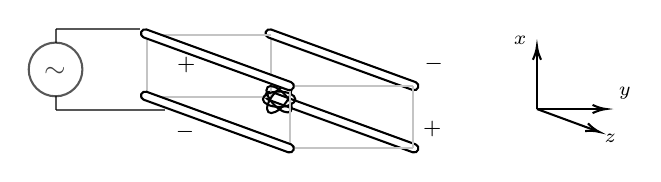
\begin{tikzpicture}[x=0.75pt,y=0.75pt,yscale=-1,xscale=1]
%uncomment if require: \path (0,81); %set diagram left start at 0, and has height of 81

%Rounded Rect [id:dp026469557108133812] 
\draw  [fill={rgb, 255:red, 255; green, 255; blue, 255 }  ,fill opacity=1 ] (125.31,46.91) .. controls (125.69,45.85) and (126.85,45.31) .. (127.91,45.69) -- (197.55,71.04) .. controls (198.6,71.42) and (199.14,72.59) .. (198.76,73.64) -- (198.76,73.64) .. controls (198.38,74.69) and (197.21,75.24) .. (196.16,74.85) -- (126.52,49.51) .. controls (125.47,49.12) and (124.92,47.96) .. (125.31,46.91) -- cycle ;
%Straight Lines [id:da3371385641661644] 
\draw [color={rgb, 255:red, 196; green, 196; blue, 196 }  ,draw opacity=1 ]   (127.91,48.35) -- (127.91,16.69) ;
%Straight Lines [id:da26074727807001774] 
\draw    (256,54) -- (287.37,54) ;
\draw [shift={(289.37,54)}, rotate = 180] [color={rgb, 255:red, 0; green, 0; blue, 0 }  ][line width=0.75]    (6.56,-1.97) .. controls (4.17,-0.84) and (1.99,-0.18) .. (0,0) .. controls (1.99,0.18) and (4.17,0.84) .. (6.56,1.97)   ;
%Straight Lines [id:da32746521719983357] 
\draw    (256,54) -- (256,25.71) ;
\draw [shift={(256,23.71)}, rotate = 90] [color={rgb, 255:red, 0; green, 0; blue, 0 }  ][line width=0.75]    (6.56,-1.97) .. controls (4.17,-0.84) and (1.99,-0.18) .. (0,0) .. controls (1.99,0.18) and (4.17,0.84) .. (6.56,1.97)   ;
%Straight Lines [id:da3165592785302246] 
\draw    (256,54) -- (284.16,64.35) ;
\draw [shift={(286.03,65.04)}, rotate = 200.19] [color={rgb, 255:red, 0; green, 0; blue, 0 }  ][line width=0.75]    (6.56,-1.97) .. controls (4.17,-0.84) and (1.99,-0.18) .. (0,0) .. controls (1.99,0.18) and (4.17,0.84) .. (6.56,1.97)   ;
%Rounded Rect [id:dp23162296971612728] 
\draw  [fill={rgb, 255:red, 255; green, 255; blue, 255 }  ,fill opacity=1 ] (125.31,16.91) .. controls (125.69,15.85) and (126.85,15.31) .. (127.91,15.69) -- (197.55,41.04) .. controls (198.6,41.42) and (199.14,42.59) .. (198.76,43.64) -- (198.76,43.64) .. controls (198.38,44.69) and (197.21,45.24) .. (196.16,44.85) -- (126.52,19.51) .. controls (125.47,19.12) and (124.92,17.96) .. (125.31,16.91) -- cycle ;
%Straight Lines [id:da7801497985171296] 
\draw [color={rgb, 255:red, 196; green, 196; blue, 196 }  ,draw opacity=1 ]   (68.87,18.35) -- (127.91,18.35) ;
%Straight Lines [id:da18932681466243861] 
\draw [color={rgb, 255:red, 196; green, 196; blue, 196 }  ,draw opacity=1 ]   (68.87,48.35) -- (127.91,48.35) ;
%Straight Lines [id:da12487858602452251] 
\draw [color={rgb, 255:red, 196; green, 196; blue, 196 }  ,draw opacity=1 ]   (137.16,72.85) -- (196.2,72.85) ;
%Straight Lines [id:da7561068891818322] 
\draw [color={rgb, 255:red, 196; green, 196; blue, 196 }  ,draw opacity=1 ]   (137.12,42.85) -- (196.16,42.85) ;
%Straight Lines [id:da36016830120348087] 
\draw [color={rgb, 255:red, 196; green, 196; blue, 196 }  ,draw opacity=1 ]   (67.91,48.35) -- (67.91,16.69) ;
%Straight Lines [id:da6626175855941887] 
\draw [color={rgb, 255:red, 196; green, 196; blue, 196 }  ,draw opacity=1 ]   (196.16,72.85) -- (196.16,42.85) ;
%Shape: Ellipse [id:dp4879513077667338] 
\draw   (123.97,49.28) .. controls (123.97,47.25) and (127.46,45.6) .. (131.77,45.6) .. controls (136.08,45.6) and (139.58,47.25) .. (139.58,49.28) .. controls (139.58,51.32) and (136.08,52.97) .. (131.77,52.97) .. controls (127.46,52.97) and (123.97,51.32) .. (123.97,49.28) -- cycle ;
%Shape: Ellipse [id:dp6977784877320135] 
\draw   (126.61,55.48) .. controls (125.17,54.14) and (126.31,50.27) .. (129.16,46.85) .. controls (132.02,43.42) and (135.5,41.74) .. (136.94,43.09) .. controls (138.38,44.43) and (137.24,48.3) .. (134.38,51.72) .. controls (131.53,55.15) and (128.05,56.83) .. (126.61,55.48) -- cycle ;
%Shape: Ellipse [id:dp4347278984290077] 
\draw   (126.2,43.5) .. controls (127.54,42.05) and (131.13,43.46) .. (134.21,46.65) .. controls (137.29,49.85) and (138.7,53.62) .. (137.35,55.07) .. controls (136,56.52) and (132.42,55.11) .. (129.34,51.92) .. controls (126.26,48.72) and (124.85,44.95) .. (126.2,43.5) -- cycle ;

%Straight Lines [id:da9283418522076294] 
\draw [color={rgb, 255:red, 196; green, 196; blue, 196 }  ,draw opacity=1 ]   (137.16,73.85) -- (137.16,42.2) ;
%Rounded Rect [id:dp4934943713792619] 
\draw  [fill={rgb, 255:red, 255; green, 255; blue, 255 }  ,fill opacity=1 ] (65.31,16.91) .. controls (65.69,15.85) and (66.85,15.31) .. (67.91,15.69) -- (137.55,41.04) .. controls (138.6,41.42) and (139.14,42.59) .. (138.76,43.64) -- (138.76,43.64) .. controls (138.38,44.69) and (137.21,45.24) .. (136.16,44.85) -- (66.52,19.51) .. controls (65.47,19.12) and (64.92,17.96) .. (65.31,16.91) -- cycle ;
%Rounded Rect [id:dp8209197314293472] 
\draw  [fill={rgb, 255:red, 255; green, 255; blue, 255 }  ,fill opacity=1 ] (65.31,46.91) .. controls (65.69,45.85) and (66.85,45.31) .. (67.91,45.69) -- (137.55,71.04) .. controls (138.6,71.42) and (139.14,72.59) .. (138.76,73.64) -- (138.76,73.64) .. controls (138.38,74.69) and (137.21,75.24) .. (136.16,74.85) -- (66.52,49.51) .. controls (65.47,49.12) and (64.92,47.96) .. (65.31,46.91) -- cycle ;
%Shape: Circle [id:dp9266584324169199] 
\draw  [color={rgb, 255:red, 0; green, 0; blue, 0 }  ,draw opacity=0.66 ] (11.13,34.93) .. controls (11.13,27.79) and (16.92,22) .. (24.07,22) .. controls (31.21,22) and (37,27.79) .. (37,34.93) .. controls (37,42.08) and (31.21,47.87) .. (24.07,47.87) .. controls (16.92,47.87) and (11.13,42.08) .. (11.13,34.93) -- cycle ;
%Straight Lines [id:da6054328790639063] 
\draw [color={rgb, 255:red, 0; green, 0; blue, 0 }  ,draw opacity=0.66 ]   (24.07,22) -- (24.07,15.53) ;
%Straight Lines [id:da8018312921143852] 
\draw [color={rgb, 255:red, 0; green, 0; blue, 0 }  ,draw opacity=0.66 ]   (24.07,15.53) -- (64.67,15.53) ;
%Straight Lines [id:da3703100332961291] 
\draw [color={rgb, 255:red, 0; green, 0; blue, 0 }  ,draw opacity=0.66 ]   (24.07,54.33) -- (24.07,47.87) ;
%Straight Lines [id:da6734660603789357] 
\draw [color={rgb, 255:red, 0; green, 0; blue, 0 }  ,draw opacity=0.66 ]   (24.07,54.33) -- (76.67,54.33) ;

% Text Node
\draw (243.33,17.6) node [anchor=north west][inner sep=0.75pt]  [font=\scriptsize]  {$x$};
% Text Node
\draw (294,42.07) node [anchor=north west][inner sep=0.75pt]  [font=\scriptsize]  {$y$};
% Text Node
\draw (287.13,64.73) node [anchor=north west][inner sep=0.75pt]  [font=\scriptsize]  {$z$};
% Text Node
\draw (81.13,27.53) node [anchor=north west][inner sep=0.75pt]  [font=\footnotesize]  {$+$};
% Text Node
\draw (199.6,58.2) node [anchor=north west][inner sep=0.75pt]  [font=\footnotesize]  {$+$};
% Text Node
\draw (80.53,59.93) node [anchor=north west][inner sep=0.75pt]  [font=\footnotesize]  {$-$};
% Text Node
\draw (200.4,26.8) node [anchor=north west][inner sep=0.75pt]  [font=\footnotesize]  {$-$};
% Text Node
\draw (17.0,32.53) node [anchor=north west][inner sep=0.75pt]  [color={rgb, 255:red, 0; green, 0; blue, 0 }  ,opacity=0.75 ]  {$\sim$};


\end{tikzpicture}

}
\end{center}
\end{tcolorbox}

Notice that the described system has three relevant length-scales:
\begin{itemize}   
    \item the typical atomic radius, which can be approximated with the Bohr radius of outer electron $\tilde{a}_0$:
    \begin{equation*}
    \tilde{a_0} \simeq \frac{n^2}{Z_{\text{eff}}} a_0 =
\frac{4^2}{2}\frac{4\pi \varepsilon_0 \hbar}{m e^2} \simeq 0.42 ~\text{nm}, 
    \end{equation*}
    where $a_0$ is the Hydrogen Bohr radius.
    
    \item the wavelength of the laser light
    $$\lambda_L = \frac{2\pi c}{\omega_L} \in \big( \underbrace{100~\text{nm}}_{UV}, \underbrace{1~\mu\text{m}}_{UV} \big)$$

    \item uncertainty in the atom position $\Delta z_{CM}$, which clearly depends on the trapping potential; considering an harmonic potential along the $z$ direction, we have
    $$V(z_{CM}) = \frac{1}{2}m_A\omega_\text{trap}^2z^2$$
    where $m_A$ is the mass of the atom/ion (for Ca$^+$, $m_\text{Ca} \simeq 40\;m_\text{proton}$) and $\omega_T$ is the trap harmonic frequency. Typical traps have $\omega_T/2\pi \in (0.1 \sim 10)$ MHz. \\
    To estimate $\Delta z_{CM}$, one has to start form the Hamiltonian of the harmonic oscillator
    $$\bar{H} = \frac{\hat{P}^2}{2m_A} + \frac{1}{2}m_A\omega_T^2\hat{z}^2 =
    \hbar\omega_T\left(\hat{a}^\dag \hat{a} +\frac{1}{2}\right),$$
    where the ladder operators 
    \begin{equation*}
    \hat{z} = \sqrt{\frac{\hbar}{2m_A\omega_T}}\left(\hat{a}+\hat{a}^\dag\right)
    \qquad \text{and} \qquad 
    \hat{P} = \sqrt{\frac{\hbar m_A\omega_T}{2}}i\left(\hat{a}^\dag-\hat{a}\right) 
    \end{equation*}
    are introduced. If we assume that the center-of-mass is in the ground state of the harmonic oscillator, then
    \begin{align*}
        \bra{0}\hat{z}\ket{0} = 
        \sqrt{\frac{\hbar}{2m_A\omega_T}}
        \big( \langle \hat{a}\rangle + \langle \hat{a}^\dag\rangle \big)
        =0
    \end{align*}
    and its variance is
    \begin{align*}
        \Delta \vec{z} & = \sqrt{\bra{0} \hat{z}^2\ket{0} - \bra{0}\hat{z}\ket{0}^2} = \\
        & =
        \sqrt{\frac{\hbar}{2m_A\omega_T}
        \left(
        \cancel{\langle \hat{a}^2\rangle}
        + \cancel{\langle \hat{a}^\dag \hat{a} \rangle}
        + \underbrace{\langle \hat{a} \hat{a}^\dag
        \rangle}_{=1}
        +\cancel{\langle {a^\dag}^2\rangle}
        \right) =
        }\\
        & = \sqrt{\frac{\hbar}{2m_A\omega_T}} = 
        \sqrt{\frac{h}{2m_A(\omega_T/2\pi)}}
    \end{align*}
    Inserting the parameters for Ca$^+$, we expect $\Delta \vec{z}$ to be in the range $10-100$ nm. 
\end{itemize}
To summarize, the involved length-scales are: 
\begin{align*}
\text{atom size} ~\tilde{a}_0 \qquad \quad & 1 ~\text{nm,} \\
\text{laser wavelength} ~\lambda_L \qquad \quad  &400~\text{nm}, 850~\text{nm}\\ 
\text{position uncertainty} ~\Delta \vec{z} \qquad \quad & 10-100~\text{nm.}
\end{align*}
Supported by those values, it is reasonable to consider from now on that
\begin{align*}
    \underbrace{\lambda_L \quad \gg \quad \Delta z }_{\eta\;\ll\;1} \quad \gg \quad  \tilde{a}_0. 
\end{align*}

\begin{center}
\tikzset{every picture/.style={line width=0.75pt}} %set default line width to 0.75pt        

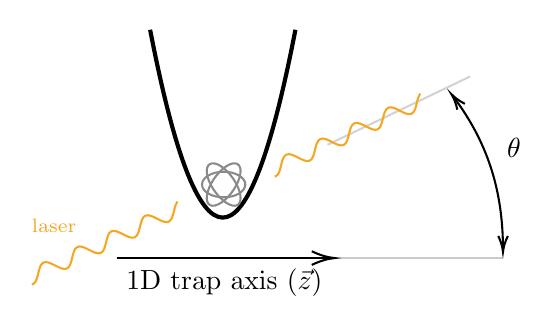
\begin{tikzpicture}[x=0.75pt,y=0.75pt,yscale=-1,xscale=1]
%uncomment if require: \path (0,144); %set diagram left start at 0, and has height of 144

%Straight Lines [id:da8108693484794903] 
\draw [color={rgb, 255:red, 203; green, 203; blue, 203 }  ,draw opacity=1 ][fill={rgb, 255:red, 174; green, 174; blue, 174 }  ,fill opacity=1 ]   (234.02,113) -- (134.02,113) ;
%Shape: Parabola [id:dp46790086230322614] 
\draw  [line width=1.5]  (64.02,3) .. controls (87.35,123.68) and (110.68,123.68) .. (134.02,3) ;
%Shape: Wave [id:dp01051452251292273] 
\draw  [color={rgb, 255:red, 245; green, 166; blue, 35 }  ,draw opacity=1 ] (7.04,125.74) .. controls (7.22,125.71) and (7.39,125.65) .. (7.56,125.58) .. controls (9.04,124.9) and (9.56,122.68) .. (10.11,120.36) .. controls (10.66,118.04) and (11.19,115.83) .. (12.67,115.15) .. controls (14.15,114.47) and (16.17,115.51) .. (18.29,116.6) .. controls (20.41,117.69) and (22.43,118.73) .. (23.91,118.05) .. controls (25.39,117.37) and (25.91,115.16) .. (26.46,112.84) .. controls (27.01,110.52) and (27.54,108.3) .. (29.02,107.62) .. controls (30.5,106.94) and (32.52,107.98) .. (34.64,109.07) .. controls (36.76,110.17) and (38.78,111.2) .. (40.26,110.52) .. controls (41.74,109.84) and (42.26,107.63) .. (42.81,105.31) .. controls (43.36,102.99) and (43.89,100.78) .. (45.37,100.1) .. controls (46.85,99.42) and (48.87,100.45) .. (50.99,101.55) .. controls (53.11,102.64) and (55.13,103.68) .. (56.61,102.99) .. controls (58.09,102.31) and (58.62,100.1) .. (59.16,97.78) .. controls (59.71,95.46) and (60.24,93.25) .. (61.72,92.57) .. controls (63.2,91.89) and (65.22,92.93) .. (67.34,94.02) .. controls (69.46,95.11) and (71.48,96.15) .. (72.96,95.47) .. controls (74.44,94.79) and (74.97,92.57) .. (75.51,90.25) .. controls (75.93,88.48) and (76.34,86.77) .. (77.17,85.76) ;
%Shape: Ellipse [id:dp6481733802903992] 
\draw  [color={rgb, 255:red, 138; green, 138; blue, 138 }  ,draw opacity=1 ] (89.02,77.57) .. controls (89.02,74.17) and (93.68,71.41) .. (99.44,71.41) .. controls (105.2,71.41) and (109.87,74.17) .. (109.87,77.57) .. controls (109.87,80.97) and (105.2,83.73) .. (99.44,83.73) .. controls (93.68,83.73) and (89.02,80.97) .. (89.02,77.57) -- cycle ;
%Shape: Ellipse [id:dp35194775511886456] 
\draw  [color={rgb, 255:red, 138; green, 138; blue, 138 }  ,draw opacity=1 ] (92.07,68.32) .. controls (93.99,65.91) and (98.84,68.1) .. (102.91,73.21) .. controls (106.99,78.32) and (108.73,84.42) .. (106.82,86.82) .. controls (104.9,89.23) and (100.04,87.04) .. (95.97,81.93) .. controls (91.9,76.82) and (90.15,70.72) .. (92.07,68.32) -- cycle ;
%Shape: Ellipse [id:dp24347781150229186] 
\draw  [color={rgb, 255:red, 138; green, 138; blue, 138 }  ,draw opacity=1 ] (92.07,86.82) .. controls (90.15,84.42) and (91.9,78.32) .. (95.97,73.21) .. controls (100.04,68.1) and (104.9,65.91) .. (106.82,68.32) .. controls (108.73,70.72) and (106.99,76.82) .. (102.92,81.93) .. controls (98.84,87.04) and (93.99,89.23) .. (92.07,86.82) -- cycle ;
%Straight Lines [id:da38657252406973086] 
\draw    (47.85,113) -- (150.82,113) ;
\draw [shift={(152.82,113)}, rotate = 180] [color={rgb, 255:red, 0; green, 0; blue, 0 }  ][line width=0.75]    (10.93,-3.29) .. controls (6.95,-1.4) and (3.31,-0.3) .. (0,0) .. controls (3.31,0.3) and (6.95,1.4) .. (10.93,3.29)   ;
%Straight Lines [id:da07907601069000136] 
\draw [color={rgb, 255:red, 211; green, 211; blue, 211 }  ,draw opacity=1 ][fill={rgb, 255:red, 174; green, 174; blue, 174 }  ,fill opacity=1 ]   (218.17,25.53) -- (149.52,58.4) ;
%Shape: Wave [id:dp41883931883450887] 
\draw  [color={rgb, 255:red, 245; green, 166; blue, 35 }  ,draw opacity=1 ] (124.04,73.74) .. controls (124.22,73.71) and (124.39,73.65) .. (124.56,73.58) .. controls (126.04,72.9) and (126.56,70.68) .. (127.11,68.36) .. controls (127.66,66.04) and (128.19,63.83) .. (129.67,63.15) .. controls (131.15,62.47) and (133.17,63.51) .. (135.29,64.6) .. controls (137.41,65.69) and (139.43,66.73) .. (140.91,66.05) .. controls (142.39,65.37) and (142.91,63.16) .. (143.46,60.84) .. controls (144.01,58.52) and (144.54,56.3) .. (146.02,55.62) .. controls (147.5,54.94) and (149.52,55.98) .. (151.64,57.07) .. controls (153.76,58.17) and (155.78,59.2) .. (157.26,58.52) .. controls (158.74,57.84) and (159.26,55.63) .. (159.81,53.31) .. controls (160.36,50.99) and (160.89,48.78) .. (162.37,48.1) .. controls (163.85,47.42) and (165.87,48.45) .. (167.99,49.55) .. controls (170.11,50.64) and (172.13,51.68) .. (173.61,50.99) .. controls (175.09,50.31) and (175.62,48.1) .. (176.16,45.78) .. controls (176.71,43.46) and (177.24,41.25) .. (178.72,40.57) .. controls (180.2,39.89) and (182.22,40.93) .. (184.34,42.02) .. controls (186.46,43.11) and (188.48,44.15) .. (189.96,43.47) .. controls (191.44,42.79) and (191.97,40.57) .. (192.51,38.25) .. controls (192.93,36.48) and (193.34,34.77) .. (194.17,33.76) ;
%Curve Lines [id:da7472332865435621] 
\draw    (210.54,35.83) .. controls (227.65,58.78) and (233.92,82.25) .. (234.02,108.4) ;
\draw [shift={(234.02,110)}, rotate = 270.33] [color={rgb, 255:red, 0; green, 0; blue, 0 }  ][line width=0.75]    (7.65,-2.3) .. controls (4.86,-0.97) and (2.31,-0.21) .. (0,0) .. controls (2.31,0.21) and (4.86,0.98) .. (7.65,2.3)   ;
\draw [shift={(209.17,34.03)}, rotate = 52.37] [color={rgb, 255:red, 0; green, 0; blue, 0 }  ][line width=0.75]    (7.65,-2.3) .. controls (4.86,-0.97) and (2.31,-0.21) .. (0,0) .. controls (2.31,0.21) and (4.86,0.98) .. (7.65,2.3)   ;

% Text Node
\draw (5.52,92.5) node [anchor=north west][inner sep=0.75pt]  [font=\scriptsize,color={rgb, 255:red, 245; green, 166; blue, 35 }  ,opacity=1 ] [align=left] {laser};
% Text Node
\draw (51.02,116.77) node [anchor=north west][inner sep=0.75pt]   [align=left] {1D trap axis ($\displaystyle \vec{z}$)};
% Text Node
\draw (234.52,53.9) node [anchor=north west][inner sep=0.75pt]    {$\theta $};


\end{tikzpicture}

\end{center}

One can define $\eta$ as the \textit{Lamb-Dicke parameter}, which is practically the ratio between atom ground-state packet size (confinement dependent) and laser wavelength
\begin{equation*}
\eta = \Delta\vec{z}\cdot\vec{k} =
\frac{2\pi\Delta z}{\lambda}\cos\theta,
\end{equation*}
with $\theta$ being the angle between the laser and trap (1D direction). The \textit{Lamb-Dicke regime} corresponds to the condition in which $\eta \ll 1$.

%\textbf{Remark}: In Innsbruck they use $\eta = 1/20$. In general, a bigger value of $\eta$ leads to a bad approximations. $\eta \sim 0.1$ is still good. On the other hand, a smaller value of $\eta$ slows down the dynamics of our system. 

Let us go back to the trapped atom system under the latest assumptions.
The contributions to the Hamiltonian are: 
\begin{align*}
H^A_{rel} &= \hbar \omega_{eg} \ket{e}\bra{e} \qquad \qquad \text{atom relative coordinate,} \\
H_{CoM}^A &= \hbar \omega_{T} \hat{a}^\dag \hat{a} + \cancel{\frac{1}{2}} \qquad  \text{atom center-of-mass coordinate,} \\
H_{AL} &= - \hat{\vec{d}} \cdot \hat{\vec{E}}(\hat{\vec{r}}_{CoM}) \qquad \qquad \text{atom-light interaction.} 
\end{align*}
$H_{CoM}^A$ can be considered as the ``phonon" Hamiltonian, while in the last expression we have taken the electric field operator in the center-of-mass coordinate because of $\Delta z\gg a_0$. In particular, 
$$\hat{\vec{d}} = \vec{d}_{eg}\ket{e}\bra{g} + \vec{d}^*_{eg}\ket{g}\bra{e} \;,$$
\begin{equation*}
\hat{\vec{E}}(\vec{r}_{CoM}) = \sum_{k\lambda} \sqrt{\frac{\hbar\omega_k}{2\varepsilon_0}}\vec\epsilon_{\lambda} \, 2 \mathfrak{Im}\left(u_{\vec{k},\lambda}(\hat{\vec{r}}_{CoM})\hat{a}_{\vec{k},\lambda}\right).
\end{equation*}
Considering a coherent light (laser) ($\vec{k}, \lambda$), the radiation is described by the Fock state
$$\ket{\psi_L} = \ket{0} \otimes ... \otimes \ket{0} \otimes \ket{\alpha_{\vec{k},\lambda}} \otimes \ket{0} \otimes ... \otimes \ket{0}$$
and therefore
\begin{flalign*}
{\bra{\psi_L} \hat{\vec{E}}\ket{\psi_L}(\hat{\vec{r}}_{CoM})} = \vec{\mathcal{E}}\cos\left(c|\vec{k}|t-\vec{k}\cdot\hat{\vec{r}}\right) =  \vec{\mathcal{E}}\cos\left(ckt-kz\cos\theta \right), 
\end{flalign*}
where in the last equation one uses the fact that the trap is tight in $x$ and $y$, $\Rightarrow \hat{\vec{r}} = (0\;\;0\;\;\hat{z})$ (no motion is allowed in xy).


Introducing the usual Rabi frequency $\Omega = \dfrac{\vec{d}_{eg} \cdot \vec{\mathcal{E}}}{\hbar}$, the effective Hamiltonian of atom-light interaction is 
\begin{equation}
H_{AL}^{\text{eff}} = \hbar\Omega\ket{e}\bra{g}
    \cos\left(ckt-kz\cos\theta\right)
    + \text{h.c.}
    \label{eq:effective-atomlight-ham}
\end{equation}
Collecting all these considerations, the full Hamiltonian in the laboratory frame is
\begin{equation*}
H^{lab} = \hbar\omega_{eg}\ket{e}\bra{e}
\;+\;
\hbar\omega_Ta^\dag a 
\;+\;
\left(
\hbar\Omega \ket{e}\bra{g}\cos\left(ckt-kz\cos\theta\right) + \text{h.c.}
\right)
\end{equation*}

Switching to a rotating frame with laser frequency $\omega_L = ck$, and requiring that $\Omega,\Delta \ll \omega_{eg}, \omega_L$, the Hamiltonian is
\begin{equation*}
H^{rot} = - \hbar \Delta
\ket{e}\bra{e} +
\hbar\omega_Ta^\dag a +
\frac{\hbar\Omega}{2}e^{-i k \hat{z}\cos\theta} \ket{e}\bra{g} +
\cancel{V(t)} + \text{h.c.}
\end{equation*}
where we have set $\Delta\equiv\omega_L-\omega_{eg}$ and $V(t)$ cancels out if we assume the timescale separation $\Omega, \Delta, \omega_T \ll \omega_L$. \\
At this point, one can observe that 
$$k\hat{z} \cos\theta = k \sqrt{\frac{\hbar}{2m_A\omega_T}}(a+a^\dag) \cos\theta =
(\Delta z k \cos\theta)(a+a^\dag) = \eta (a^\dag + a)  \;\;.$$

\noindent Being $\eta$ sufficiently small (due to Lamb-Dicke regime), the expansion up to second order is
$$e^{-i\eta(a^\dag+a)}\simeq 1- i\eta(a^\dag +a) + O(\eta^2) \;\;,$$ from which
\begin{align*}
\Rightarrow H^{rot} = &
-\hbar \Delta\ket{e}\bra{e}
+ \frac{\hbar\Omega}{2}
\underbrace{\left( \ket{e}\bra{g}+\ket{g}\bra{e} \right)}_{\sigma^x} +
\tag*{internal degrees of freedom only} \\
& + \hbar\omega_Ta^\dag a +
\tag*{phononic contribution only}\\
& + \eta\frac{\hbar\Omega}{2}
\underbrace{\left(-i\ket{e}\bra{g}+i\ket{g}\bra{e}\right)}
_{-\sigma_y}
\left( a + a^\dag \right) +
\tag*{Lamb-Dicke effective coupling (sidebands)}\\
&+ \mathcal{O}(\eta^2) \tag*{higher-order corrections/sidebands}
\end{align*}
Finally, one can write
\begin{align}
 H^{rot} &= -\hbar \Delta\ket{e}\bra{e} +
\hbar\omega_Ta^\dag a +
\frac{\hbar\Omega}{2}\sigma^x +
\eta\frac{\hbar\Omega}{2}\sigma^y
\left( a + a^\dag \right)
\end{align}

To understand the physics described by this Hamiltonian, let us start from the situation in which $\Omega = \omega_L =0 $: in this case only the bare spectrum of the atomic system survives. Instead, when the laser light is turned on, any generic level $\ket{g,n}$ couples to $\ket{e, n-1}, \ket{e,n}$ and $\ket{e, n+1}$, as shown in the following figure. 

\begin{center}


\tikzset{every picture/.style={line width=0.75pt}} %set default line width to 0.75pt        

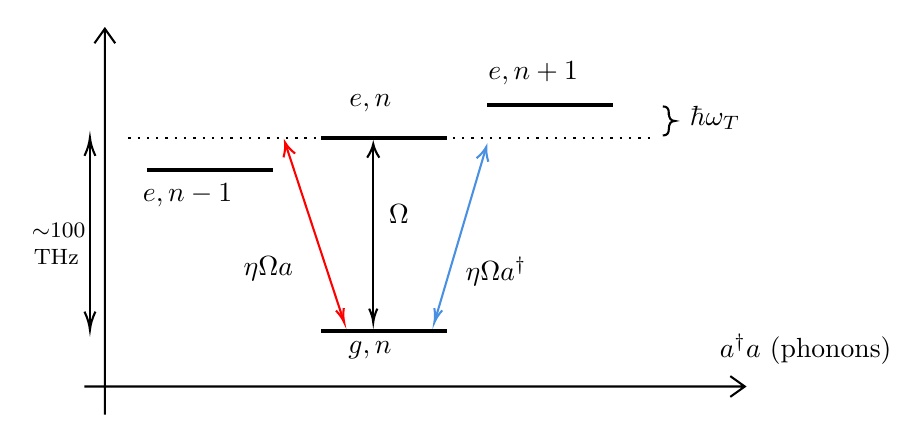
\begin{tikzpicture}[x=0.75pt,y=0.75pt,yscale=-1,xscale=1]
%uncomment if require: \path (0,199); %set diagram left start at 0, and has height of 199

%Shape: Axis 2D [id:dp6304689266356812] 
\draw  (37.83,176.32) -- (356.01,176.32)(47.68,3.94) -- (47.68,189.88) (349.01,171.32) -- (356.01,176.32) -- (349.01,181.32) (42.68,10.94) -- (47.68,3.94) -- (52.68,10.94)  ;
%Straight Lines [id:da9096429015684652] 
\draw [line width=1.5]    (68,72) -- (128.47,72) ;
%Straight Lines [id:da10599775473097062] 
\draw [line width=1.5]    (152,149.5) -- (212.47,149.5) ;
%Straight Lines [id:da5859149964722625] 
\draw [line width=1.5]    (152,56.5) -- (212.47,56.5) ;
%Straight Lines [id:da32072281915513823] 
\draw [line width=1.5]    (232,40.5) -- (292.47,40.5) ;
%Straight Lines [id:da09610392103973153] 
\draw    (40.5,58.44) -- (40.5,147) ;
\draw [shift={(40.5,149)}, rotate = 270] [color={rgb, 255:red, 0; green, 0; blue, 0 }  ][line width=0.75]    (8.74,-2.63) .. controls (5.56,-1.12) and (2.65,-0.24) .. (0,0) .. controls (2.65,0.24) and (5.56,1.12) .. (8.74,2.63)   ;
\draw [shift={(40.5,56.44)}, rotate = 90] [color={rgb, 255:red, 0; green, 0; blue, 0 }  ][line width=0.75]    (8.74,-2.63) .. controls (5.56,-1.12) and (2.65,-0.24) .. (0,0) .. controls (2.65,0.24) and (5.56,1.12) .. (8.74,2.63)   ;
%Straight Lines [id:da3310136117207533] 
\draw [color={rgb, 255:red, 255; green, 0; blue, 0 }  ,draw opacity=1 ]   (135.12,60.67) -- (162.34,143.47) ;
\draw [shift={(162.97,145.38)}, rotate = 251.81] [color={rgb, 255:red, 255; green, 0; blue, 0 }  ,draw opacity=1 ][line width=0.75]    (6.56,-1.97) .. controls (4.17,-0.84) and (1.99,-0.18) .. (0,0) .. controls (1.99,0.18) and (4.17,0.84) .. (6.56,1.97)   ;
\draw [shift={(134.5,58.77)}, rotate = 71.81] [color={rgb, 255:red, 255; green, 0; blue, 0 }  ,draw opacity=1 ][line width=0.75]    (6.56,-2.94) .. controls (4.17,-1.38) and (1.99,-0.4) .. (0,0) .. controls (1.99,0.4) and (4.17,1.38) .. (6.56,2.94)   ;
%Straight Lines [id:da10284525377100584] 
\draw [color={rgb, 255:red, 74; green, 144; blue, 226 }  ,draw opacity=1 ]   (230.9,62.79) -- (207.03,143.46) ;
\draw [shift={(206.47,145.38)}, rotate = 286.48] [color={rgb, 255:red, 74; green, 144; blue, 226 }  ,draw opacity=1 ][line width=0.75]    (6.56,-1.97) .. controls (4.17,-0.84) and (1.99,-0.18) .. (0,0) .. controls (1.99,0.18) and (4.17,0.84) .. (6.56,1.97)   ;
\draw [shift={(231.47,60.88)}, rotate = 106.48] [color={rgb, 255:red, 74; green, 144; blue, 226 }  ,draw opacity=1 ][line width=0.75]    (6.56,-2.94) .. controls (4.17,-1.38) and (1.99,-0.4) .. (0,0) .. controls (1.99,0.4) and (4.17,1.38) .. (6.56,2.94)   ;
%Straight Lines [id:da5949199879144775] 
\draw    (177,61.5) -- (177,143.38) ;
\draw [shift={(177,145.38)}, rotate = 270] [color={rgb, 255:red, 0; green, 0; blue, 0 }  ][line width=0.75]    (6.56,-1.97) .. controls (4.17,-0.84) and (1.99,-0.18) .. (0,0) .. controls (1.99,0.18) and (4.17,0.84) .. (6.56,1.97)   ;
\draw [shift={(177,59.5)}, rotate = 90] [color={rgb, 255:red, 0; green, 0; blue, 0 }  ][line width=0.75]    (6.56,-2.94) .. controls (4.17,-1.38) and (1.99,-0.4) .. (0,0) .. controls (1.99,0.4) and (4.17,1.38) .. (6.56,2.94)   ;
%Straight Lines [id:da5656279166859981] 
\draw  [dash pattern={on 0.84pt off 2.51pt}]  (59,56.5) -- (310.97,56.5) ;
%Shape: Brace [id:dp5779107364872813] 
\draw   (316.5,55.38) .. controls (318.42,55.38) and (319.38,54.42) .. (319.38,52.49) -- (319.38,52.49) .. controls (319.38,49.75) and (320.34,48.38) .. (322.26,48.38) .. controls (320.34,48.38) and (319.38,47.01) .. (319.38,44.26)(319.38,45.49) -- (319.38,44.26) .. controls (319.38,42.34) and (318.42,41.38) .. (316.5,41.38) ;

% Text Node
\draw (64.5,76.9) node [anchor=north west][inner sep=0.75pt]    {$\ket{e,n-1}$};
% Text Node
\draw (163.5,153.4) node [anchor=north west][inner sep=0.75pt]    {$\ket{g,n}$};
% Text Node
\draw (164,34.4) node [anchor=north west][inner sep=0.75pt]    {$\ket{e,n}$};
% Text Node
\draw (231,18.4) node [anchor=north west][inner sep=0.75pt]    {$\ket{e,n+1}$};
% Text Node
\draw (342.5,149.4) node [anchor=north west][inner sep=0.75pt]    {$a^{\dagger } a$ (phonons)};
% Text Node
\draw (11,90.5) node [anchor=north west][inner sep=0.75pt]  [font=\footnotesize] [align=left] {\begin{minipage}[lt]{17.68pt}\setlength\topsep{0pt}
\begin{center}
$\sim$100\\THz
\end{center}

\end{minipage}};
% Text Node
\draw (220,112.4) node [anchor=north west][inner sep=0.75pt]    {$\eta\Omega a^{\dagger }$};
% Text Node
\draw (113,112.4) node [anchor=north west][inner sep=0.75pt]    {$\eta\Omega a$};
% Text Node
\draw (183,87.4) node [anchor=north west][inner sep=0.75pt]    {$\Omega $};
% Text Node
\draw (328,39.9) node [anchor=north west][inner sep=0.75pt]    {$\hbar\omega _{T}$};


\end{tikzpicture}

\includegraphics[height=4cm]{img/dicke-red-plot.png}
\end{center}

\subsubsection{Sideband coupling}

There are three coupling sub-regimes, depending on the frequency to which the laser is tuned and the are represented in figure \ref{fig:sideband-coupling}.We analyze each case separately.
\begin{figure}[H]
    \centering
    

\tikzset{every picture/.style={line width=0.75pt}} %set default line width to 0.75pt        

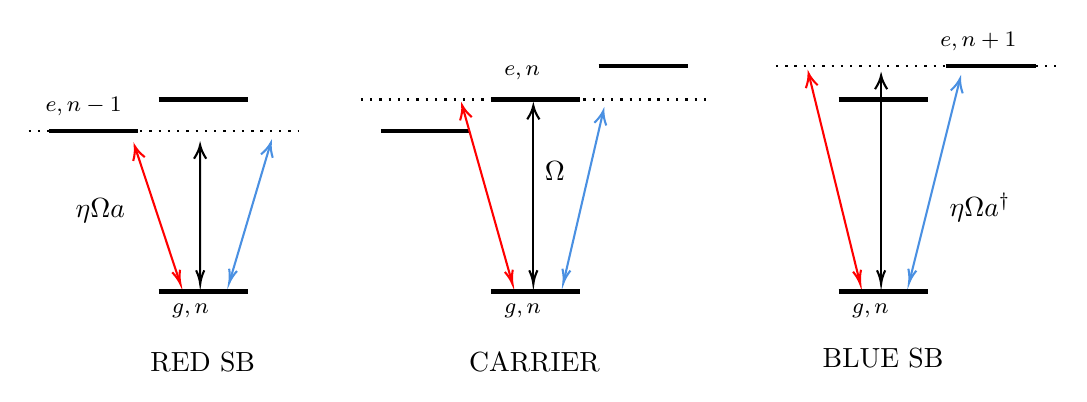
\begin{tikzpicture}[x=0.75pt,y=0.75pt,yscale=-1,xscale=1]
%uncomment if require: \path (0,176); %set diagram left start at 0, and has height of 176

%Straight Lines [id:da14028990751255077] 
\draw [line width=1.5]    (9.63,51.5) -- (52.63,51.5) ;
%Straight Lines [id:da11175967521568253] 
\draw [color={rgb, 255:red, 255; green, 0; blue, 0 }  ,draw opacity=1 ]   (51.71,60.87) -- (72.46,123.48) ;
\draw [shift={(73.09,125.38)}, rotate = 251.66] [color={rgb, 255:red, 255; green, 0; blue, 0 }  ,draw opacity=1 ][line width=0.75]    (6.56,-1.97) .. controls (4.17,-0.84) and (1.99,-0.18) .. (0,0) .. controls (1.99,0.18) and (4.17,0.84) .. (6.56,1.97)   ;
\draw [shift={(51.08,58.97)}, rotate = 71.66] [color={rgb, 255:red, 255; green, 0; blue, 0 }  ,draw opacity=1 ][line width=0.75]    (6.56,-2.94) .. controls (4.17,-1.38) and (1.99,-0.4) .. (0,0) .. controls (1.99,0.4) and (4.17,1.38) .. (6.56,2.94)   ;
%Straight Lines [id:da29434586221130576] 
\draw [color={rgb, 255:red, 74; green, 144; blue, 226 }  ,draw opacity=1 ]   (116.05,59.38) -- (97.16,122.96) ;
\draw [shift={(96.59,124.88)}, rotate = 286.55] [color={rgb, 255:red, 74; green, 144; blue, 226 }  ,draw opacity=1 ][line width=0.75]    (6.56,-1.97) .. controls (4.17,-0.84) and (1.99,-0.18) .. (0,0) .. controls (1.99,0.18) and (4.17,0.84) .. (6.56,1.97)   ;
\draw [shift={(116.62,57.47)}, rotate = 106.55] [color={rgb, 255:red, 74; green, 144; blue, 226 }  ,draw opacity=1 ][line width=0.75]    (6.56,-2.94) .. controls (4.17,-1.38) and (1.99,-0.4) .. (0,0) .. controls (1.99,0.4) and (4.17,1.38) .. (6.56,2.94)   ;
%Straight Lines [id:da035858476752611446] 
\draw    (82.58,60.47) -- (82.62,123.38) ;
\draw [shift={(82.63,125.38)}, rotate = 269.96] [color={rgb, 255:red, 0; green, 0; blue, 0 }  ][line width=0.75]    (6.56,-1.97) .. controls (4.17,-0.84) and (1.99,-0.18) .. (0,0) .. controls (1.99,0.18) and (4.17,0.84) .. (6.56,1.97)   ;
\draw [shift={(82.58,58.47)}, rotate = 89.96] [color={rgb, 255:red, 0; green, 0; blue, 0 }  ][line width=0.75]    (6.56,-2.94) .. controls (4.17,-1.38) and (1.99,-0.4) .. (0,0) .. controls (1.99,0.4) and (4.17,1.38) .. (6.56,2.94)   ;
%Straight Lines [id:da790497420088156] 
\draw  [dash pattern={on 0.84pt off 2.51pt}]  (0,51.5) -- (130.38,51.5) ;
%Straight Lines [id:da9900161263211081] 
\draw [line width=1.5]    (62.63,36.5) -- (105.63,36.5) ;
%Straight Lines [id:da18120661834702578] 
\draw [line width=1.5]    (62.63,129) -- (105.63,129) ;
%Straight Lines [id:da3376964100631521] 
\draw [line width=1.5]    (169.63,51.5) -- (212.63,51.5) ;
%Straight Lines [id:da217953660823897] 
\draw [color={rgb, 255:red, 255; green, 0; blue, 0 }  ,draw opacity=1 ]   (209.42,41.39) -- (232.55,123.45) ;
\draw [shift={(233.09,125.38)}, rotate = 254.26] [color={rgb, 255:red, 255; green, 0; blue, 0 }  ,draw opacity=1 ][line width=0.75]    (6.56,-1.97) .. controls (4.17,-0.84) and (1.99,-0.18) .. (0,0) .. controls (1.99,0.18) and (4.17,0.84) .. (6.56,1.97)   ;
\draw [shift={(208.88,39.47)}, rotate = 74.26] [color={rgb, 255:red, 255; green, 0; blue, 0 }  ,draw opacity=1 ][line width=0.75]    (6.56,-2.94) .. controls (4.17,-1.38) and (1.99,-0.4) .. (0,0) .. controls (1.99,0.4) and (4.17,1.38) .. (6.56,2.94)   ;
%Straight Lines [id:da6608184995861122] 
\draw [color={rgb, 255:red, 74; green, 144; blue, 226 }  ,draw opacity=1 ]   (276.42,43.91) -- (258.04,122.93) ;
\draw [shift={(257.59,124.88)}, rotate = 283.09] [color={rgb, 255:red, 74; green, 144; blue, 226 }  ,draw opacity=1 ][line width=0.75]    (6.56,-1.97) .. controls (4.17,-0.84) and (1.99,-0.18) .. (0,0) .. controls (1.99,0.18) and (4.17,0.84) .. (6.56,1.97)   ;
\draw [shift={(276.88,41.97)}, rotate = 103.09] [color={rgb, 255:red, 74; green, 144; blue, 226 }  ,draw opacity=1 ][line width=0.75]    (6.56,-2.94) .. controls (4.17,-1.38) and (1.99,-0.4) .. (0,0) .. controls (1.99,0.4) and (4.17,1.38) .. (6.56,2.94)   ;
%Straight Lines [id:da13619447520920935] 
\draw    (243.13,41.5) -- (243.13,123.38) ;
\draw [shift={(243.13,125.38)}, rotate = 270] [color={rgb, 255:red, 0; green, 0; blue, 0 }  ][line width=0.75]    (6.56,-1.97) .. controls (4.17,-0.84) and (1.99,-0.18) .. (0,0) .. controls (1.99,0.18) and (4.17,0.84) .. (6.56,1.97)   ;
\draw [shift={(243.13,39.5)}, rotate = 90] [color={rgb, 255:red, 0; green, 0; blue, 0 }  ][line width=0.75]    (6.56,-2.94) .. controls (4.17,-1.38) and (1.99,-0.4) .. (0,0) .. controls (1.99,0.4) and (4.17,1.38) .. (6.56,2.94)   ;
%Straight Lines [id:da8825274475937802] 
\draw  [dash pattern={on 0.84pt off 2.51pt}]  (160,36.5) -- (328.25,36.5) ;
%Straight Lines [id:da4376283057123779] 
\draw [line width=1.5]    (222.63,36.5) -- (265.63,36.5) ;
%Straight Lines [id:da3655084631996305] 
\draw [line width=1.5]    (222.63,129) -- (265.63,129) ;
%Straight Lines [id:da36481720214842805] 
\draw [line width=1.5]    (274.63,20.5) -- (317.63,20.5) ;
%Straight Lines [id:da14498321918646662] 
\draw [color={rgb, 255:red, 255; green, 0; blue, 0 }  ,draw opacity=1 ]   (376.21,25.91) -- (400.16,123.43) ;
\draw [shift={(400.64,125.38)}, rotate = 256.2] [color={rgb, 255:red, 255; green, 0; blue, 0 }  ,draw opacity=1 ][line width=0.75]    (6.56,-1.97) .. controls (4.17,-0.84) and (1.99,-0.18) .. (0,0) .. controls (1.99,0.18) and (4.17,0.84) .. (6.56,1.97)   ;
\draw [shift={(375.73,23.97)}, rotate = 76.2] [color={rgb, 255:red, 255; green, 0; blue, 0 }  ,draw opacity=1 ][line width=0.75]    (6.56,-2.94) .. controls (4.17,-1.38) and (1.99,-0.4) .. (0,0) .. controls (1.99,0.4) and (4.17,1.38) .. (6.56,2.94)   ;
%Straight Lines [id:da7981259927773865] 
\draw [color={rgb, 255:red, 74; green, 144; blue, 226 }  ,draw opacity=1 ]   (448.25,28.41) -- (424.63,122.93) ;
\draw [shift={(424.14,124.88)}, rotate = 284.03] [color={rgb, 255:red, 74; green, 144; blue, 226 }  ,draw opacity=1 ][line width=0.75]    (6.56,-1.97) .. controls (4.17,-0.84) and (1.99,-0.18) .. (0,0) .. controls (1.99,0.18) and (4.17,0.84) .. (6.56,1.97)   ;
\draw [shift={(448.73,26.47)}, rotate = 104.03] [color={rgb, 255:red, 74; green, 144; blue, 226 }  ,draw opacity=1 ][line width=0.75]    (6.56,-2.94) .. controls (4.17,-1.38) and (1.99,-0.4) .. (0,0) .. controls (1.99,0.4) and (4.17,1.38) .. (6.56,2.94)   ;
%Straight Lines [id:da035896781940746525] 
\draw    (410.68,26.97) -- (410.68,123.38) ;
\draw [shift={(410.68,125.38)}, rotate = 270] [color={rgb, 255:red, 0; green, 0; blue, 0 }  ][line width=0.75]    (6.56,-1.97) .. controls (4.17,-0.84) and (1.99,-0.18) .. (0,0) .. controls (1.99,0.18) and (4.17,0.84) .. (6.56,1.97)   ;
\draw [shift={(410.68,24.97)}, rotate = 90] [color={rgb, 255:red, 0; green, 0; blue, 0 }  ][line width=0.75]    (6.56,-2.94) .. controls (4.17,-1.38) and (1.99,-0.4) .. (0,0) .. controls (1.99,0.4) and (4.17,1.38) .. (6.56,2.94)   ;
%Straight Lines [id:da07315183718019935] 
\draw  [dash pattern={on 0.84pt off 2.51pt}]  (360,20.5) -- (495.8,20.5) ;
%Straight Lines [id:da886475154974947] 
\draw [line width=1.5]    (390.18,36.5) -- (433.18,36.5) ;
%Straight Lines [id:da021693587273391435] 
\draw [line width=1.5]    (390.18,129) -- (433.18,129) ;
%Straight Lines [id:da5682832670921795] 
\draw [line width=1.5]    (442.18,20.5) -- (485.18,20.5) ;

% Text Node
\draw (6.63,33.9) node [anchor=north west][inner sep=0.75pt]  [font=\footnotesize]  {$\ket{e,n-1}$};
% Text Node
\draw (67.63,133.4) node [anchor=north west][inner sep=0.75pt]  [font=\footnotesize]  {$\ket{g,n}$};
% Text Node
\draw (21.13,82.9) node [anchor=north west][inner sep=0.75pt]    {$\eta\Omega a$};
% Text Node
\draw (227.63,133.4) node [anchor=north west][inner sep=0.75pt]  [font=\footnotesize]  {$\ket{g,n}$};
% Text Node
\draw (227.63,18.9) node [anchor=north west][inner sep=0.75pt]  [font=\footnotesize]  {$\ket{e,n}$};
% Text Node
\draw (247.13,64.9) node [anchor=north west][inner sep=0.75pt]    {$\Omega $};
% Text Node
\draw (395.18,133.4) node [anchor=north west][inner sep=0.75pt]  [font=\footnotesize]  {$\ket{g,n}$};
% Text Node
\draw (437.68,2.4) node [anchor=north west][inner sep=0.75pt]  [font=\footnotesize]  {$\ket{e,n+1}$};
% Text Node
\draw (442.18,79.9) node [anchor=north west][inner sep=0.75pt]    {$\eta\Omega a^{\dagger }$};
% Text Node
\draw (83.84,157) node [anchor=north] [inner sep=0.75pt]   [align=left] {RED SB};
% Text Node
\draw (243.64,157) node [anchor=north] [inner sep=0.75pt]   [align=left] {CARRIER};
% Text Node
\draw (411.64,155) node [anchor=north] [inner sep=0.75pt]   [align=left] {BLUE SB};


\end{tikzpicture}

    \caption{The three sub-regimes of sideband coupling.}
    \label{fig:sideband-coupling}
\end{figure}


\begin{enumerate}
    \item[1)] \textbf{Carrier resonance} ($\Delta = 0$, or at least $\Delta \ll \omega_T$)\\
    In this regime, the laser is resonant with the direct transition $\Delta \ll \omega_T$ (and weak $\eta\Omega \ll \omega_T$). In particular, there is no coupling between $\ket{g,n}$ and $\ket{e, n\pm 1}$, because by construction $|\omega_T \pm \Delta| \approx \omega_T \;\gg\; \eta\Omega$ . The Hamiltonian is approximately
\begin{equation*}
H_\text{carrier} = \hbar\omega_Ta^\dag a
\;-\;
\hbar\Delta\ket{e}\bra{e}
\;+\;
\frac{\hbar\Omega}{2}\sigma^x 
\sim \begin{pmatrix}
0&\Omega/2 \\
\Omega/2&\omega_T
\end{pmatrix}
\end{equation*}
having used the basis $\{\ket{g,n}, \ket{e, n+1}\}$ to write the matrix elements.

\item[2)] \textbf{Red sideband} ($\Delta \simeq -\omega_T$, or at least $|\omega_L - (\omega_{eg}-\omega_T)| \ll \omega_T$) \\ 
In this case, the laser is resonant with $\omega_{eg} -\omega_T$. We also require that $\Omega \ll \omega_T$.
The denomination ``red" is due to the fact that laser is detuned to a lower frequency (hence more ``red") than carrier. In practice, we ignore the direct and the blue transition, considering only couples $\ket{g,n} \longleftrightarrow \ket{e, n-1}$, as shown in the following figure. 
\begin{center}
    

\tikzset{every picture/.style={line width=0.75pt}} %set default line width to 0.75pt        

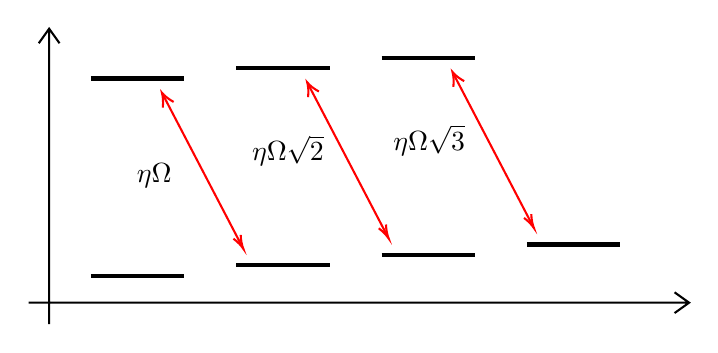
\begin{tikzpicture}[x=0.75pt,y=0.75pt,yscale=-1,xscale=1]
%uncomment if require: \path (0,158); %set diagram left start at 0, and has height of 158

%Shape: Axis 2D [id:dp8431562196616039] 
\draw  (0,138) -- (318.17,138)(9.85,6) -- (9.85,148.38) (311.17,133) -- (318.17,138) -- (311.17,143) (4.85,13) -- (9.85,6) -- (14.85,13)  ;
%Straight Lines [id:da5651762429163826] 
\draw [line width=1.5]    (30,125) -- (75,125) ;
%Straight Lines [id:da16666480216181523] 
\draw [color={rgb, 255:red, 255; green, 0; blue, 0 }  ,draw opacity=1 ]   (65.09,38.6) -- (102.5,110.29) ;
\draw [shift={(103.42,112.06)}, rotate = 242.44] [color={rgb, 255:red, 255; green, 0; blue, 0 }  ,draw opacity=1 ][line width=0.75]    (6.56,-1.97) .. controls (4.17,-0.84) and (1.99,-0.18) .. (0,0) .. controls (1.99,0.18) and (4.17,0.84) .. (6.56,1.97)   ;
\draw [shift={(64.17,36.82)}, rotate = 62.44] [color={rgb, 255:red, 255; green, 0; blue, 0 }  ,draw opacity=1 ][line width=0.75]    (6.56,-2.94) .. controls (4.17,-1.38) and (1.99,-0.4) .. (0,0) .. controls (1.99,0.4) and (4.17,1.38) .. (6.56,2.94)   ;
%Straight Lines [id:da9273633131691024] 
\draw [line width=1.5]    (30,30) -- (75,30) ;
%Straight Lines [id:da8337269026387355] 
\draw [line width=1.5]    (100,120) -- (145,120) ;
%Straight Lines [id:da41032876729774204] 
\draw [color={rgb, 255:red, 255; green, 0; blue, 0 }  ,draw opacity=1 ]   (135.09,33.6) -- (172.5,105.29) ;
\draw [shift={(173.42,107.06)}, rotate = 242.44] [color={rgb, 255:red, 255; green, 0; blue, 0 }  ,draw opacity=1 ][line width=0.75]    (6.56,-1.97) .. controls (4.17,-0.84) and (1.99,-0.18) .. (0,0) .. controls (1.99,0.18) and (4.17,0.84) .. (6.56,1.97)   ;
\draw [shift={(134.17,31.82)}, rotate = 62.44] [color={rgb, 255:red, 255; green, 0; blue, 0 }  ,draw opacity=1 ][line width=0.75]    (6.56,-2.94) .. controls (4.17,-1.38) and (1.99,-0.4) .. (0,0) .. controls (1.99,0.4) and (4.17,1.38) .. (6.56,2.94)   ;
%Straight Lines [id:da7310518864520119] 
\draw [line width=1.5]    (100,25) -- (145,25) ;
%Straight Lines [id:da3116124591913111] 
\draw [line width=1.5]    (170,115) -- (215,115) ;
%Straight Lines [id:da12641083556456256] 
\draw [color={rgb, 255:red, 255; green, 0; blue, 0 }  ,draw opacity=1 ]   (205.09,28.6) -- (242.5,100.29) ;
\draw [shift={(243.42,102.06)}, rotate = 242.44] [color={rgb, 255:red, 255; green, 0; blue, 0 }  ,draw opacity=1 ][line width=0.75]    (6.56,-1.97) .. controls (4.17,-0.84) and (1.99,-0.18) .. (0,0) .. controls (1.99,0.18) and (4.17,0.84) .. (6.56,1.97)   ;
\draw [shift={(204.17,26.82)}, rotate = 62.44] [color={rgb, 255:red, 255; green, 0; blue, 0 }  ,draw opacity=1 ][line width=0.75]    (6.56,-2.94) .. controls (4.17,-1.38) and (1.99,-0.4) .. (0,0) .. controls (1.99,0.4) and (4.17,1.38) .. (6.56,2.94)   ;
%Straight Lines [id:da5597533072353611] 
\draw [line width=1.5]    (170,20) -- (215,20) ;
%Straight Lines [id:da38450978230425914] 
\draw [line width=1.5]    (240,110) -- (285,110) ;

% Text Node
\draw (50.67,69.46) node [anchor=north west][inner sep=0.75pt]    {$\eta\Omega $};
% Text Node
\draw (106.17,55.96) node [anchor=north west][inner sep=0.75pt]    {$\eta\Omega \sqrt{2}$};
% Text Node
\draw (174.17,50.96) node [anchor=north west][inner sep=0.75pt]    {$\eta\Omega \sqrt{3}$};


\end{tikzpicture}

\end{center}
The Hamiltonian in this case is
\begin{equation*}
\Rightarrow H_{\text{red}} = \hbar\omega_Ta^\dag a
-
\hbar\Delta\ket{e}\bra{e}
+
\eta\frac{\hbar\Omega}{2}
\left(-i\sigma_+a+i\sigma_-a^\dag\right), 
\end{equation*}
which is the Jaynes-Cummings model (between phonon and level $e$). The difference with respect to the cavity is that the last contribution can be turned off, as the system is controlled by the laser.

\item[3)] \textbf{Blue sideband} ($\Delta \simeq +\omega_T$, or at least $|\omega_L - (\omega_{eg}+\omega_T)| \ll \omega_T$) \\
In this case, the laser is resonant with $\omega_{eg} +\omega_T$. We also require that $\Omega \ll \omega_T$. \\
We can check the energy scales for typical optical systems:
$$\underbrace{|\omega_L -(\omega_{eg}+\omega_T)|}_
{\sim \text{kHz}}
\ll
\underbrace{\omega_T}_{\text{MHz}},$$
The Hamiltonian in this regime is 
\begin{equation*}
\Rightarrow H_{\text{blue}} = \hbar\omega_Ta^\dag a
-
\hbar\Delta\ket{e}\bra{e}
+
\frac{\eta\hbar\Omega}{2}
\left(-i\sigma_+a^\dag+i\sigma_-a\right).
\end{equation*}
It is called ``anti"-Jaynes-Cummings model. 

\begin{center}


\tikzset{every picture/.style={line width=0.75pt}} %set default line width to 0.75pt        

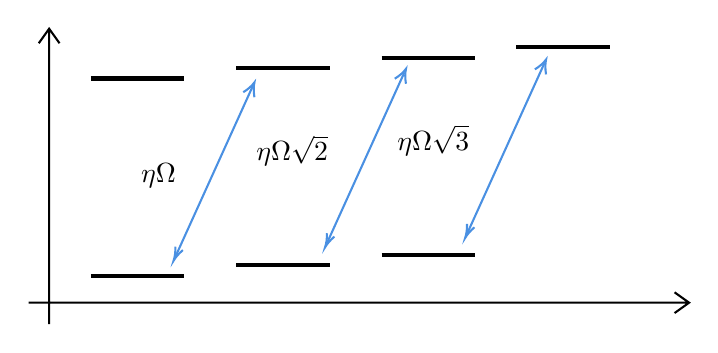
\begin{tikzpicture}[x=0.75pt,y=0.75pt,yscale=-1,xscale=1]
%uncomment if require: \path (0,158); %set diagram left start at 0, and has height of 158

%Shape: Axis 2D [id:dp15618946884319262] 
\draw  (0,138) -- (318.17,138)(9.85,6) -- (9.85,148.38) (311.17,133) -- (318.17,138) -- (311.17,143) (4.85,13) -- (9.85,6) -- (14.85,13)  ;
%Straight Lines [id:da5633161593663423] 
\draw [line width=1.5]    (30,125) -- (75,125) ;
%Straight Lines [id:da6891482979787938] 
\draw [color={rgb, 255:red, 74; green, 144; blue, 226 }  ,draw opacity=1 ]   (107.95,33.65) -- (70.6,116.01) ;
\draw [shift={(69.77,117.83)}, rotate = 294.39] [color={rgb, 255:red, 74; green, 144; blue, 226 }  ,draw opacity=1 ][line width=0.75]    (6.56,-1.97) .. controls (4.17,-0.84) and (1.99,-0.18) .. (0,0) .. controls (1.99,0.18) and (4.17,0.84) .. (6.56,1.97)   ;
\draw [shift={(108.77,31.83)}, rotate = 114.39] [color={rgb, 255:red, 74; green, 144; blue, 226 }  ,draw opacity=1 ][line width=0.75]    (6.56,-2.94) .. controls (4.17,-1.38) and (1.99,-0.4) .. (0,0) .. controls (1.99,0.4) and (4.17,1.38) .. (6.56,2.94)   ;
%Straight Lines [id:da5552335178166578] 
\draw [line width=1.5]    (30,30) -- (75,30) ;
%Straight Lines [id:da6891740634193314] 
\draw [line width=1.5]    (100,120) -- (145,120) ;
%Straight Lines [id:da5661851604865566] 
\draw [line width=1.5]    (100,25) -- (145,25) ;
%Straight Lines [id:da6022612634715885] 
\draw [line width=1.5]    (170,115) -- (215,115) ;
%Straight Lines [id:da9393350496146184] 
\draw [line width=1.5]    (170,20) -- (215,20) ;
%Straight Lines [id:da2934899407823195] 
\draw [line width=1.5]    (235,15) -- (280,15) ;
%Straight Lines [id:da3308284960238893] 
\draw [color={rgb, 255:red, 74; green, 144; blue, 226 }  ,draw opacity=1 ]   (180.95,27.15) -- (143.6,109.51) ;
\draw [shift={(142.77,111.33)}, rotate = 294.39] [color={rgb, 255:red, 74; green, 144; blue, 226 }  ,draw opacity=1 ][line width=0.75]    (6.56,-1.97) .. controls (4.17,-0.84) and (1.99,-0.18) .. (0,0) .. controls (1.99,0.18) and (4.17,0.84) .. (6.56,1.97)   ;
\draw [shift={(181.77,25.33)}, rotate = 114.39] [color={rgb, 255:red, 74; green, 144; blue, 226 }  ,draw opacity=1 ][line width=0.75]    (6.56,-2.94) .. controls (4.17,-1.38) and (1.99,-0.4) .. (0,0) .. controls (1.99,0.4) and (4.17,1.38) .. (6.56,2.94)   ;
%Straight Lines [id:da6178275915895299] 
\draw [color={rgb, 255:red, 74; green, 144; blue, 226 }  ,draw opacity=1 ]   (248.45,22.65) -- (211.1,105.01) ;
\draw [shift={(210.27,106.83)}, rotate = 294.39] [color={rgb, 255:red, 74; green, 144; blue, 226 }  ,draw opacity=1 ][line width=0.75]    (6.56,-1.97) .. controls (4.17,-0.84) and (1.99,-0.18) .. (0,0) .. controls (1.99,0.18) and (4.17,0.84) .. (6.56,1.97)   ;
\draw [shift={(249.27,20.83)}, rotate = 114.39] [color={rgb, 255:red, 74; green, 144; blue, 226 }  ,draw opacity=1 ][line width=0.75]    (6.56,-2.94) .. controls (4.17,-1.38) and (1.99,-0.4) .. (0,0) .. controls (1.99,0.4) and (4.17,1.38) .. (6.56,2.94)   ;

% Text Node
\draw (52.67,69.46) node [anchor=north west][inner sep=0.75pt]    {$\eta\Omega $};
% Text Node
\draw (108.17,55.96) node [anchor=north west][inner sep=0.75pt]    {$\eta\Omega \sqrt{2}$};
% Text Node
\draw (176.17,50.96) node [anchor=north west][inner sep=0.75pt]    {$\eta\Omega \sqrt{3}$};


\end{tikzpicture}

\end{center}

\end{enumerate}


\begin{tcolorbox} [breakable, enhanced]
\textbf{{Some observations about the effective Rabi frequency}} \\
Frequencies mismatch is an issue when designing multi-qubit gates on ion traps: asynchrony requires perfect cooling (or any other workaround). Indeed, if one considers traps in the order of MHz, the temperatures must be really low: 1 MHz $\simeq 48\mu$K. \\
The red sideband can be efficiently used to cool-down atom vibrations, as it reduces the effective number of phonon spontaneously (\textit{phonon drift}).
\end{tcolorbox}


\section{Two atoms in a linear trap}
%\marginnote{This is actually a path towards ion-qubit\\ (trapped ion)\\ quantum computation.}

\begin{center}
    

\tikzset{every picture/.style={line width=0.75pt}} %set default line width to 0.75pt        

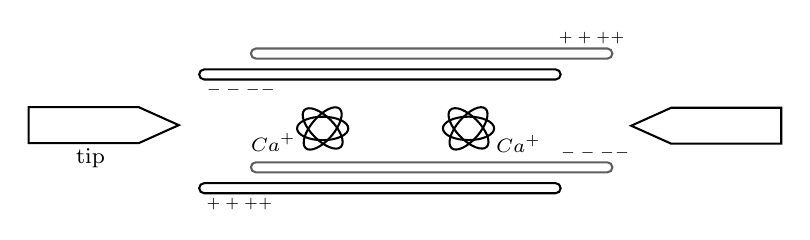
\begin{tikzpicture}[x=0.75pt,y=0.75pt,yscale=-1,xscale=1]
%uncomment if require: \path (0,109); %set diagram left start at 0, and has height of 109

%Pentagon Arrow [id:dp794168685774739] 
\draw   (4,43.62) -- (57.06,43.62) -- (76.3,52.26) -- (57.06,60.91) -- (4,60.91) -- cycle ;
%Shape: Ellipse [id:dp04697411659497153] 
\draw   (133.29,53.85) .. controls (133.29,50.74) and (138.81,48.21) .. (145.63,48.21) .. controls (152.45,48.21) and (157.98,50.74) .. (157.98,53.85) .. controls (157.98,56.97) and (152.45,59.5) .. (145.63,59.5) .. controls (138.81,59.5) and (133.29,56.97) .. (133.29,53.85) -- cycle ;
%Shape: Ellipse [id:dp8824898187216484] 
\draw   (137.46,63.35) .. controls (135.19,61.28) and (136.99,55.36) .. (141.51,50.12) .. controls (146.02,44.88) and (151.52,42.3) .. (153.8,44.36) .. controls (156.08,46.42) and (154.27,52.35) .. (149.76,57.59) .. controls (145.25,62.83) and (139.74,65.41) .. (137.46,63.35) -- cycle ;
%Shape: Ellipse [id:dp13173681950698235] 
\draw   (136.81,44.99) .. controls (138.94,42.77) and (144.62,44.93) .. (149.49,49.82) .. controls (154.36,54.71) and (156.58,60.49) .. (154.45,62.71) .. controls (152.32,64.94) and (146.65,62.78) .. (141.78,57.89) .. controls (136.91,52.99) and (134.69,47.22) .. (136.81,44.99) -- cycle ;

%Rounded Rect [id:dp743242906420414] 
\draw  [fill={rgb, 255:red, 255; green, 255; blue, 255 }  ,fill opacity=1 ] (260.29,27.84) .. controls (260.29,26.49) and (259.2,25.41) .. (257.86,25.41) -- (88.56,25.41) .. controls (87.22,25.41) and (86.13,26.49) .. (86.13,27.84) -- (86.13,27.84) .. controls (86.13,29.18) and (87.22,30.27) .. (88.56,30.27) -- (257.86,30.27) .. controls (259.2,30.27) and (260.29,29.18) .. (260.29,27.84) -- cycle ;
%Shape: Ellipse [id:dp96829721697133] 
\draw   (203.55,53.82) .. controls (203.55,50.7) and (209.08,48.17) .. (215.9,48.17) .. controls (222.72,48.17) and (228.24,50.7) .. (228.24,53.82) .. controls (228.24,56.94) and (222.72,59.47) .. (215.9,59.47) .. controls (209.08,59.47) and (203.55,56.94) .. (203.55,53.82) -- cycle ;
%Shape: Ellipse [id:dp14893138861753885] 
\draw   (207.73,63.31) .. controls (205.45,61.25) and (207.26,55.33) .. (211.77,50.08) .. controls (216.28,44.84) and (221.79,42.26) .. (224.07,44.33) .. controls (226.35,46.39) and (224.54,52.31) .. (220.03,57.56) .. controls (215.51,62.8) and (210.01,65.38) .. (207.73,63.31) -- cycle ;
%Shape: Ellipse [id:dp9581768791328901] 
\draw   (207.08,44.96) .. controls (209.21,42.73) and (214.88,44.89) .. (219.75,49.79) .. controls (224.62,54.68) and (226.84,60.45) .. (224.72,62.68) .. controls (222.59,64.91) and (216.91,62.75) .. (212.04,57.85) .. controls (207.17,52.96) and (204.95,47.19) .. (207.08,44.96) -- cycle ;

%Rounded Rect [id:dp04110522752915269] 
\draw  [color={rgb, 255:red, 95; green, 95; blue, 95 }  ,draw opacity=1 ][fill={rgb, 255:red, 255; green, 255; blue, 255 }  ,fill opacity=1 ] (285.21,17.78) .. controls (285.21,16.44) and (284.12,15.35) .. (282.78,15.35) -- (113.48,15.35) .. controls (112.14,15.35) and (111.05,16.44) .. (111.05,17.78) -- (111.05,17.78) .. controls (111.05,19.12) and (112.14,20.21) .. (113.48,20.21) -- (282.78,20.21) .. controls (284.12,20.21) and (285.21,19.12) .. (285.21,17.78) -- cycle ;
%Pentagon Arrow [id:dp587265405222459] 
\draw   (366.57,61.18) -- (313.52,61.18) -- (294.27,52.54) -- (313.52,43.89) -- (366.57,43.89) -- cycle ;
%Rounded Rect [id:dp2560808105145962] 
\draw  [fill={rgb, 255:red, 255; green, 255; blue, 255 }  ,fill opacity=1 ] (260.29,82.64) .. controls (260.29,81.3) and (259.2,80.21) .. (257.86,80.21) -- (88.56,80.21) .. controls (87.22,80.21) and (86.13,81.3) .. (86.13,82.64) -- (86.13,82.64) .. controls (86.13,83.98) and (87.22,85.07) .. (88.56,85.07) -- (257.86,85.07) .. controls (259.2,85.07) and (260.29,83.98) .. (260.29,82.64) -- cycle ;
%Rounded Rect [id:dp3099051608838199] 
\draw  [color={rgb, 255:red, 95; green, 95; blue, 95 }  ,draw opacity=1 ][fill={rgb, 255:red, 255; green, 255; blue, 255 }  ,fill opacity=1 ] (285.21,72.59) .. controls (285.21,71.25) and (284.12,70.16) .. (282.78,70.16) -- (113.48,70.16) .. controls (112.14,70.16) and (111.05,71.25) .. (111.05,72.59) -- (111.05,72.59) .. controls (111.05,73.93) and (112.14,75.02) .. (113.48,75.02) -- (282.78,75.02) .. controls (284.12,75.02) and (285.21,73.93) .. (285.21,72.59) -- cycle ;

% Text Node
\draw (88.13,86.04) node [anchor=north west][inner sep=0.75pt]  [font=\tiny]  {$++++$};
% Text Node
\draw (258.72,61.45) node [anchor=north west][inner sep=0.75pt]  [font=\tiny]  {$----$};
% Text Node
\draw (109.55,54.79) node [anchor=north west][inner sep=0.75pt]  [font=\scriptsize]  {$Ca^{+}$};
% Text Node
\draw (257.77,5.8) node [anchor=north west][inner sep=0.75pt]  [font=\tiny]  {$++++$};
% Text Node
\draw (88.13,31.24) node [anchor=north west][inner sep=0.75pt]  [font=\tiny]  {$----$};
% Text Node
\draw (227.75,55.51) node [anchor=north west][inner sep=0.75pt]  [font=\scriptsize]  {$Ca^{+}$};
% Text Node
\draw (25.32,62.13) node [anchor=north west][inner sep=0.75pt]   [align=left] {{\footnotesize tip}};


\end{tikzpicture}

\end{center}

Consider the same trap used for the single ion (with a quadrupolar confining potential which effectively tights any atom to the $xy$ plane). If one puts two (identical) ions inside the trap, they crystallize due to their equal charge.
The Hamiltonian that describes the system is 
\begin{equation}
\label{eq:atomsharmonic}
H \;=\;
\frac{(p_1^z)^2+(p_2^z)^2}{2m}
\;+\;
\underbrace{\frac{1}{2}m\omega_T^2(z_1^2+z_2^2)}
_{\text{trap on }{z}}
\;+\;
\underbrace{\frac{e^2 Z_{\text{eff}}^2
}{4\pi \varepsilon_0|z_1-z_2|}}
_{\text{Coulomb repulsion}}
\end{equation}
In particular, $Z_{\text{eff}}=1$ for any single-ionised atom. \\ 
There is no analytical exact solution to this problem. Nevertheless, one can solve a simpler classical problem, for instance under the hypothesis of small oscillations, and prove ``a posteriori" that the solution is consistent.

The fist step is a translation of the coordinates about the \textit{classical equilibrium position}
$\bar{z}_j$:
\begin{equation*}
\hat{z}_j \rightarrow \hat{z}_j' - \bar{z}_j\mathds{1}
\end{equation*}
Notice that $\bar{z}_j$ is just a number, not an operator, and that the commutation rules are preserved, i.e. $[z_i',p_j]=[z_i,p_j]+\bar{z}\cancel{[\mathbb{1},p_j]} = [z_i,p_j]$. \\
Since the two atoms are crystallized, one can choose which atom has the greater $z_i$ coordinate and orient $\vec{z}$ such that 
$$\bar{z}_1 > \bar{z}_2 \qquad \implies \qquad \frac{1}{|z_1-z_2|} \xrightarrow[]{z_1>z_2} \frac{1}{z_1-z_2} \;\;.$$

Let us find $\bar{z}_1$ and $\bar{z}_2$.
On the hypothesis of \textit{classical equilibrium}, for a generic coordinate $q_j$ it is
\begin{align*}
\dot{p}_j = 0\qquad \implies \qquad
0 = -\dot{p}_j = \frac{\partial H}{\partial q_j}
\end{align*}
from which, in the $z_j$ coordinates,
\begin{align}
\label{eq:atomsmoments}
\frac{\partial H}{\partial z_j} \bigg\rvert_{\bar{z}_j} = 0
\;\;\Rightarrow\;\;
\begin{cases}
    m\omega_T^2\bar{z}_1 -\dfrac{e^2}{4\pi\varepsilon_0(\bar{z}_1-\bar{z}_2)^2} = 0\\
    m\omega_T^2\bar{z}_2 + \dfrac{e^2}{4\pi\varepsilon_0(\bar{z}_1-\bar{z}_2)^2} = 0
\end{cases}
\end{align}
Summing the equations, one gets easily that $\bar{z}_1=-\bar{z}_2$. Substituting back, the first equation reads
\begin{equation}
\label{eq:atomssymmetrycond}
m\omega_T^2\bar{z}_1 = \frac{e^2}{4\pi\varepsilon_0}\frac{1}{4\bar{z}_1^2}
\qquad \implies \qquad
\bar{z}_1 = 
\left( \frac{e^2}{16\pi\varepsilon_0m\omega_T^2} \right)^{1/3} = -\bar{z}_2
\end{equation}
Now we want to rewrite Eq. \ref{eq:atomsharmonic} in prime coordinates. The coordinates of the Coulombian term can be expanded for small oscillations as
\begin{equation*}
|\hat{z}_1-\hat{z}_2|^{-1} \equalexpl{$z_1>z_2$}
(\hat{z}_1-\hat{z}_2)^{-1} \simeq
\frac{\mathds{1}}{\hat{z}_1-\hat{z}_2}
-\frac{\hat{z}_1'-\hat{z}_2'}{(\bar{z}_1-\bar{z}_2)^2}
+\frac{\cancel{2}}{\cancel{2}}\frac{(\hat{z}_1'-\hat{z}_2')^2}{(\bar{z}_1-\bar{z}_2)^3}
+{O}(\hat{z}_j^{\prime\;3})
\end{equation*}
whereas the trap term requires the square of the coordinates, which is
\begin{equation*}
\hat{z}_j = \hat{z}_j' + \bar{z}_j\mathds{1}
\qquad\implies\qquad
\hat{z}_j^2 = \hat{z}_j^{\prime\;2} +
2\bar{z}_j\hat{z}_j^\prime +
\bar{z}_j^2\mathds{1} \;\;.
\end{equation*}
Shifting away the constants, one ends up with the Hamiltonian 
\begin{align}
\begin{split}
H_{\substack{\text{small} \\ \text{oscill.}}} = \; &
\frac{(p_1^z)^2+(p_2^z)^2}{2m}
\;+ \\
& +\; \frac{m\omega_T^2}{2}
    \left(
        \cancel{\bar{z}_1^2\mathds{1}} + \cancel{\bar{z}_2^2\mathds{1}}
        + 2 \bar{z}_1\hat{z}_1' + 2 \bar{z}_2\hat{z}_2'
        + \hat{z}_1^{\prime\;2} + \hat{z}_2^{\prime\;2}
    \right) \;+ \\
& +\;
\frac{e^2}{4\pi \varepsilon_0}
\left(
    \cancel{\frac{\mathds{1}}{ \hat{z}_1-\hat{z}_2 }}       - \frac{\hat{z}_1'-\hat{z}_2'}{(\hat{z}_1-\hat{z}_2)^2}
        + \frac{(\hat{z}_1'-\hat{z}_2')^2}{(\hat{z}_1-\hat{z}_2)^3}
\right)
+{O}(\hat{z}_j^{\prime\;3})
\end{split}
\end{align}
Further simplifications can be done isolating the terms by their order:
\begin{itemize}
    \item at first order in the prime coordinates, because of Equations \ref{eq:atomsmoments}
    \begin{equation*}
    (I) \qquad \longrightarrow \qquad
        \hat{z}_1' \underbrace{
            \left(
                m\omega_T^2\bar{z}_1 - \frac{e^2}{4\pi\varepsilon_0(4\bar{z}_1^2)} 
            \right)
        }_{=0} + \hat{z}_2' \underbrace{
            \left(
                m\omega_T^2\bar{z}_2 + \frac{e^2}{4\pi\varepsilon_0(4\bar{z}_2^2)} 
            \right)
        }_{=0} = 0
    \end{equation*}
    Not surprisingly... this quantity is null by construction.
    
    \item at second order
    \begin{equation*}
    (II) \qquad \longrightarrow \qquad
    \frac{m\omega_T^2}{2}
    \left( \hat{z}_1^{\prime\;2} + \hat{z}_2^{\prime\;2}  \right)
    +
    \left( \hat{z}_1^{\prime\;2} - \hat{z}_2^{\prime\;2} \right)
    {\frac{e^2}{4\pi\varepsilon_0}(\bar{z}_1-\bar{z}_2)^{-3}}
    \end{equation*}
    where, because of Eq. \ref{eq:atomssymmetrycond},
    \begin{equation*}
    \frac{e^2}{4\pi\varepsilon_0}(\bar{z}_1-\bar{z}_2)^{-3} =
    \frac{e^2}{4\pi\varepsilon_0}\frac{1}{8\bar{z}_1^3} =
    \frac{e^2}{32\pi\varepsilon_0}
    \left(
        \frac{16\pi\varepsilon_0m\omega^2_T}{e^2}
    \right) = \frac{1}{2}m\omega_T^2
    \end{equation*}
\end{itemize}
Combining the simplifications,
\begin{align}
\label{eq:atoms-harmonic-coupled}
H_{\substack{\text{small} \\ \text{oscill.}}} = 
\frac{(p_1^z)^2+(p_2^z)^2}{2m}
+
 \frac{m\omega_T^2}{2}
    \left(
        \hat{z}_1^{\prime\;2} + \hat{z}_2^{\prime\;2}
        + \left( \hat{z}_1'-\hat{z}_1' \right)^2
    \right)
    + {O}\left( z_j^3 \right)
\end{align}
This Hamiltonian describes two coupled harmonic oscillators. One can define this new set of coordinates
\begin{equation}
\text{CoM}: \begin{dcases}
Z=\frac{z_1'+z_2'}{2}\\P=p_1^z+p_2^z
\end{dcases}
\qquad \qquad 
\text{Relative}: \begin{dcases}
z=z_1-z_2\\p = \frac{p^z_1-p^z_2}{2}
\end{dcases}
\end{equation}
which inverts as
\begin{equation*}
\label{eq:inverted-coords-coupled}
p_{1,2}^z = \frac{P}{2}\pm p \qquad \qquad z'_{1,2} = Z\pm\frac{z}{2}
\end{equation*}
The terms of Equation \ref{eq:atoms-harmonic-coupled} can be written using the new coordinates
\begin{equation*}
(p_{1}^z)^2 + (p_{2}^z)^2 = \frac{P^2}{2} + 2p^2 \;,
\qquad 
(z'_1)^2 + (z'_2)^2 = 2Z^2 + \frac{z^2}{2} \;,
\qquad \text{and} \qquad
(z'_1 - z'_2)^2 = z^2.
\end{equation*}
These coordinates are really convenient, because the new Hamiltonian is the sum of two decoupled problems:
\begin{equation}
\label{eq:twoatoms-harmonic-modes}
H_{\substack{\text{small} \\ \text{oscill.}}} = 
\underbrace{\left[ \frac{P^2}{4m}+m\omega_T^2Z^2 \right]}
_{\text{CoM harmonic oscillator}}
+ 
\underbrace{\left[\frac{p^2}{m}+\frac{m\omega_T^2}{2}\left(\frac{3z^2}{2}\right)\right]}
_{\text{Stretch mode harmonic oscillator}}
+ \;\;{O}\left( z_j^3 \right)
\end{equation}


% define the dotted arrows
\def\bulletrightarrow{\hbox{$\bullet$}\kern-2pt\hbox{$\rightarrow$}}
\def\bulletleftarrow{\hbox{$\leftarrow$}\kern-2pt\hbox{$\bullet$}}


\noindent To solve this problem, one moves to the ladder operators formalism for each the two normal modes of the decoupled harmonic oscillators:
\begin{itemize}

    \item \textbf{CoM mode}
    $\qquad \left( \substack{
        \bulletrightarrow \; \; \bulletrightarrow \\ 
        \bulletleftarrow  \; \; \bulletleftarrow } \right)$
    \begin{align*}
    \begin{dcases}
        Z = \sqrt{\frac{\hbar}{4m\omega_T}}
            \left(  a_{CoM} + a_{CoM}^\dag \right)\\
        P = i\sqrt{\hbar m\omega_T}
            \left(  a_{CoM}^\dag - a_{CoM} \right)
    \end{dcases}
    \;\;\Leftrightarrow\;\; a_{CoM} = \sqrt{\frac{m\omega_T}{\hbar}}\;Z+
            i\sqrt{\frac{1}{4\hbar m\omega_T}}\;P
    \end{align*}

    \item \textbf{Stretch mode}
    $\qquad \left( \substack{ 
        \bulletrightarrow \; \; \bulletleftarrow \\
        \bulletleftarrow  \; \; \bulletrightarrow } \right)$
    \begin{align*}
    \begin{dcases}
        z = \sqrt{\frac{\hbar}{\sqrt{3}m\omega_T}}
            \left(  a_{S} + a_{S}^\dag \right)\\
        p = i\sqrt{\frac{\sqrt{3}\hbar m\omega_T}{4}}
            \left(  a_{S}^\dag - a_{S} \right)
    \end{dcases}
    \;\;\Leftrightarrow \;\;
    a_{S} = \sqrt{\frac{\sqrt{3}m\omega_T}{4\hbar}}\;z+
            i\sqrt{\frac{1}{\sqrt{3}\hbar m\omega_T}}\;p
    \end{align*}
\end{itemize}
This leads to an utterly simplified form of equation (\ref{eq:twoatoms-harmonic-modes}):
\begin{align}
\label{eq:twoatoms-ladder-harmonic-modes}
H_{\substack{\text{small} \\ \text{oscill.}}} = \hbar\omega_T
    \left( a_{CoM}^\dag a_{CoM} + \cancel{\frac{1}{2}} \right) +
    \hbar\sqrt{3}\omega_T
    \left( a_{S}^\dag a_{S} + \cancel{\frac{1}{2}} \right)
    + \cancel{\mathcal{O}\left( \dots \right)},
\end{align}
where the constant terms have been removed. We also see that the stretch mode is $\sqrt{3} \simeq 1.73$ times faster than $CoM$ mode, that is, several MHz away.

At the end of the day, one can recover the laboratory coordinates of the two atoms with $z_{1,2}=\pm\bar{z}_1+z'_{1,2} = \pm \bar{z}_1 + Z \pm \frac{z}{2}$,
\begin{equation}
\label{eq:lab-coords}
z_{1,2} =
    \pm\bar{z}
    + \sqrt{\frac{\hbar}{4m\omega_T}}
        \left( a_{CoM} + a_{CoM}^\dag \right)
    \pm \sqrt{\frac{\hbar}{4\sqrt{3}m\omega_T}}
        \left( a_S + a_S^\dag \right)
\end{equation}
and observe that their distance is orders of magnitude greater than the atom size. This means that the two atoms are sufficiently ``far away'', so one can suppose to be able to hit specifically one of them with a laser. Which is exactly what we will do!

%\begin{figure}[h!]
%\centering
%    \includegraphics[width=0.3\linewidth]{img/sketch_far_atoms.png}
%\end{figure}


\subsection{Two trapped atoms under a focused laser}

\marginnote{From now on, we will shorten $CoM$ with $C$.}
Suppose to focus a laser, say, on ion 1 (of coordinate $z_1$). The Hamiltonian of such system would be composed by the one of equation (\ref{eq:twoatoms-ladder-harmonic-modes}), plus a dipole light-atom coupling term $H_{AL} = -\vec{d}\cdot\vec{E}(\vec{r})$:
\begin{equation}
H^{lab} = 
\underbrace{
\hbar \omega_Ta_{C}^\dag a_{C}
+
\sqrt{3}\hbar\omega_Ta_S^\dag a_S
}_{\ref{eq:twoatoms-ladder-harmonic-modes}}
+ \hbar\Omega\sum_j\ket{e}\bra{e}_j + H_{AL}
\end{equation}
where
\begin{align*}
H_{AL} &= -\hbar\Omega\ket{e}\bra{g}_1
\cos\left(ckt-\cos\theta kz_1\right) + \text{h.c.}
\end{align*}
can be rewritten using equation (\ref{eq:lab-coords})
\begin{align*}
    H_{AL} = -\hbar\Omega\ket{e}\bra{g}_1 \cos
\bigg(&
    ckt -
    \underbrace{\cos\theta k\bar{z}_1}_{\phi_0}
    -\underbrace{\cos\theta k \sqrt{\frac{\hbar}{4m\omega_T}}}
        _{\eta_{C}}
    (a_{C}+a^\dag_{C}) + \\
    &-\underbrace{\cos\theta k \sqrt{\frac{\hbar}{4\sqrt{3}m\omega_T}}}
        _{\eta_{S}}
    (a_{S}+a^\dag_{S})
\bigg)
+ \text{h.c.}
\end{align*}
Consider the rotating-wave approximation 
$$|\omega_{eg}-\omega_L|,\Omega \;\ll\; \omega_{eg},\omega_L$$
and in the rotating frame, defined by the transformation
$U(t) = e^{-i\omega_L t\sum_j\ket{e}\bra{e}_j + i \phi_0}$. The Hamiltonian becomes
\begin{align*}
\begin{split}
H^{rot}_{RWA} =\; &
\hbar \overbrace{\left(\omega_{eg}-\omega_{L}\right)}
    ^{\equiv-\Delta}
\sum_j \ket{e}\bra{e}_j 
+
\hbar \omega_{T}a_{C}^\dag a_{C}
+
\sqrt{3}\hbar\omega_Ta_S^\dag a_S
+\\
& -\frac{\hbar\Omega}{2}\ket{e}\bra{g}_1
e^{-i\eta_{C}(a+a^\dag)_{C}}
e^{-i\eta_{S}(a+a^\dag)_{S}}
+ \text{h.c.}
\end{split}
\end{align*}
Using the hypothesis that the $\eta$s are small parameters (Lamb-Dicke regime)
\begin{align*}
    e^{-i\eta_{C}(a+a^\dag)_{C}}
    e^{-i\eta_{S}(a+a^\dag)_{S}}
    = 1 
    - i\eta_{C}(a_{C}+a_{C}^\dag) 
    - i\eta_{S}(a_{S}+a_{S}^\dag) 
    + \mathcal{O}(\eta^2) \;\;,
\end{align*}
the final result is
\begin{align}
\begin{split}
H^{rot}_{RWA} =\; &
-\hbar\Delta
\sum_j \ket{e}\bra{e}_j 
+
\hbar \omega_{T}a_{C}^\dag a_{C}
+
\sqrt{3}\hbar\omega_Ta_S^\dag a_S
+\\
& -\frac{\hbar\Omega}{2}\ket{e}\bra{g}_1
\left(
1 - i\eta_{C}(a_{C}+a_{C}^\dag)
- i\eta_{S}(a_{S}+a_{S}^\dag)
+{O}(\eta^2)
\right)
+ \text{h.c.}
\end{split}
\end{align}

From an experimental point of view, it would be possible to tune the laser to a specific sideband of a specific mode. Consider, for instance, the red sideband of CoM mode reported in the following figure: 
\begin{center}
    

\tikzset{every picture/.style={line width=0.75pt}} %set default line width to 0.75pt        

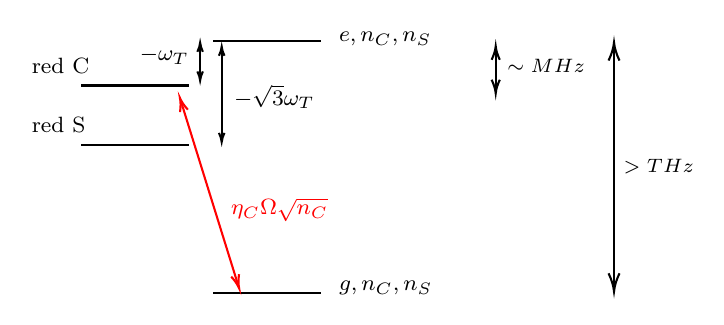
\begin{tikzpicture}[x=0.75pt,y=0.75pt,yscale=-1,xscale=1]
%uncomment if require: \path (0,146); %set diagram left start at 0, and has height of 146

%Straight Lines [id:da8993089849930328] 
\draw    (30.38,59.59) -- (82.31,59.59) ;
%Straight Lines [id:da29699103187525655] 
\draw    (30.38,30.75) -- (82.31,30.75) ;
%Straight Lines [id:da9565575071502495] 
\draw    (93.89,130.93) -- (145.83,130.93) ;
%Straight Lines [id:da38723274535804597] 
\draw    (93.89,9.5) -- (145.83,9.5) ;
%Straight Lines [id:da7230830907382644] 
\draw    (87.59,12.14) -- (87.59,26.36) ;
\draw [shift={(87.59,28.36)}, rotate = 270] [color={rgb, 255:red, 0; green, 0; blue, 0 }  ][line width=0.75]    (4.37,-1.32) .. controls (2.78,-0.56) and (1.32,-0.12) .. (0,0) .. controls (1.32,0.12) and (2.78,0.56) .. (4.37,1.32)   ;
\draw [shift={(87.59,10.14)}, rotate = 90] [color={rgb, 255:red, 0; green, 0; blue, 0 }  ][line width=0.75]    (4.37,-1.32) .. controls (2.78,-0.56) and (1.32,-0.12) .. (0,0) .. controls (1.32,0.12) and (2.78,0.56) .. (4.37,1.32)   ;
%Straight Lines [id:da7613574342882506] 
\draw    (97.98,14.06) -- (97.98,55.96) ;
\draw [shift={(97.98,57.96)}, rotate = 270] [color={rgb, 255:red, 0; green, 0; blue, 0 }  ][line width=0.75]    (4.37,-1.32) .. controls (2.78,-0.56) and (1.32,-0.12) .. (0,0) .. controls (1.32,0.12) and (2.78,0.56) .. (4.37,1.32)   ;
\draw [shift={(97.98,12.06)}, rotate = 90] [color={rgb, 255:red, 0; green, 0; blue, 0 }  ][line width=0.75]    (4.37,-1.32) .. controls (2.78,-0.56) and (1.32,-0.12) .. (0,0) .. controls (1.32,0.12) and (2.78,0.56) .. (4.37,1.32)   ;
%Straight Lines [id:da17453665512381966] 
\draw [color={rgb, 255:red, 255; green, 0; blue, 0 }  ,draw opacity=1 ]   (78.43,38.62) -- (105.81,126.62) ;
\draw [shift={(106.4,128.53)}, rotate = 252.72] [color={rgb, 255:red, 255; green, 0; blue, 0 }  ,draw opacity=1 ][line width=0.75]    (6.56,-1.97) .. controls (4.17,-0.84) and (1.99,-0.18) .. (0,0) .. controls (1.99,0.18) and (4.17,0.84) .. (6.56,1.97)   ;
\draw [shift={(77.84,36.71)}, rotate = 72.72] [color={rgb, 255:red, 255; green, 0; blue, 0 }  ,draw opacity=1 ][line width=0.75]    (6.56,-1.97) .. controls (4.17,-0.84) and (1.99,-0.18) .. (0,0) .. controls (1.99,0.18) and (4.17,0.84) .. (6.56,1.97)   ;
%Straight Lines [id:da35411700829971027] 
\draw    (287,12) -- (287,128) ;
\draw [shift={(287,130)}, rotate = 270] [color={rgb, 255:red, 0; green, 0; blue, 0 }  ][line width=0.75]    (8.74,-2.63) .. controls (5.56,-1.12) and (2.65,-0.24) .. (0,0) .. controls (2.65,0.24) and (5.56,1.12) .. (8.74,2.63)   ;
\draw [shift={(287,10)}, rotate = 90] [color={rgb, 255:red, 0; green, 0; blue, 0 }  ][line width=0.75]    (8.74,-2.63) .. controls (5.56,-1.12) and (2.65,-0.24) .. (0,0) .. controls (2.65,0.24) and (5.56,1.12) .. (8.74,2.63)   ;
%Straight Lines [id:da3640218170366485] 
\draw    (230,13.8) -- (230,32.55) ;
\draw [shift={(230,34.55)}, rotate = 270] [color={rgb, 255:red, 0; green, 0; blue, 0 }  ][line width=0.75]    (6.56,-1.97) .. controls (4.17,-0.84) and (1.99,-0.18) .. (0,0) .. controls (1.99,0.18) and (4.17,0.84) .. (6.56,1.97)   ;
\draw [shift={(230,11.8)}, rotate = 90] [color={rgb, 255:red, 0; green, 0; blue, 0 }  ][line width=0.75]    (6.56,-1.97) .. controls (4.17,-0.84) and (1.99,-0.18) .. (0,0) .. controls (1.99,0.18) and (4.17,0.84) .. (6.56,1.97)   ;

% Text Node
\draw (153,123.4) node [anchor=north west][inner sep=0.75pt]  [font=\footnotesize]  {$\ket{g,n_{C} ,n_{S}}$};
% Text Node
\draw (153,3.4) node [anchor=north west][inner sep=0.75pt]  [font=\footnotesize]  {$\ket{e,n_{C} ,n_{S}}$};
% Text Node
\draw (57,10.9) node [anchor=north west][inner sep=0.75pt]  [font=\footnotesize]  {$-\omega _{T}$};
% Text Node
\draw (102.5,28.9) node [anchor=north west][inner sep=0.75pt]  [font=\footnotesize]  {$-\sqrt{3} \omega _{T}$};
% Text Node
\draw (5,16) node [anchor=north west][inner sep=0.75pt]  [font=\footnotesize] [align=left] {red C};
% Text Node
\draw (5,44.5) node [anchor=north west][inner sep=0.75pt]  [font=\footnotesize] [align=left] {red S};
% Text Node
\draw (290,64.63) node [anchor=north west][inner sep=0.75pt]  [font=\scriptsize]  {$ >THz$};
% Text Node
\draw (234,16.43) node [anchor=north west][inner sep=0.75pt]  [font=\scriptsize]  {$\sim MHz$};
% Text Node
\draw (101,83.63) node [anchor=north west][inner sep=0.75pt]  [font=\footnotesize,color={rgb, 255:red, 255; green, 0; blue, 0 }  ,opacity=1 ]  {$\eta_C \Omega \sqrt{n_{C}}$};


\end{tikzpicture}

\end{center}

The detuning is sufficiently large to make it possible and the stretch mode will not be excited. Indeed, if
\begin{align*}
\text{KHz} \approx |\Delta + \omega_T| \ll \omega_T \approx \text{MHz}
\end{align*}
but
\begin{align*}
|\Delta\pm\sqrt{3}\omega_T| & \approx | -\omega_T \pm \sqrt{3}\omega_T| \approx\\
& \approx |\sqrt{3}\pm1|\omega_T  \;
\underbrace{\;> 0.7 \cdot \omega_T \;\approx \text{MHz}}_{ \mathclap{\text{far detuned ($\Rightarrow$ no excitation of stretch mode)}} }
\end{align*}

\noindent The Hamiltonian would be a center-of-mass (axial) phonon Jaynes-Cummings model:
\begin{align}
\begin{split}
H_{red} = & -\hbar(\omega_T +\varepsilon)
    \ket{e}\bra{e}_1 
    \;+\;
    \hbar \omega_{T}a_{C}^\dag a_{C}
    \;+ \\
& +\frac{\hbar\eta_{C}\Omega}{2}
\left( i\sigma_1^+a_{C} - i\sigma_1^-a_{C} \right)
\;\; + \text{decoupled stuff}
\end{split}
\end{align}
having defined $|\omega_L-\omega_{eg}+\omega_T| = \varepsilon \ll \omega_T$. 

\vspace{1cm}
\begin{tcolorbox}[breakable, enhanced]
\textbf{Summary}\\

Let us briefly recap the take-away message of this section. We have considered two atoms in a trap with two focused laser beams. We have found that the dynamics of the system is described by two modes.
\begin{equation*}
\text{construction}\;\; \left( \substack{
        \bulletrightarrow \; \; \bulletrightarrow \\ 
        \bulletleftarrow  \; \; \bulletleftarrow } \right)
\qquad\qquad
\text{destruction}\;\;
\left( \substack{ 
        \bulletrightarrow \; \; \bulletleftarrow \\
        \bulletleftarrow  \; \; \bulletrightarrow } \right)
\end{equation*}
which create a phonon structure, like the one seen in previous paragraphs, but separable on each mode:
\begin{center}
    

\tikzset{every picture/.style={line width=0.75pt}} %set default line width to 0.75pt        

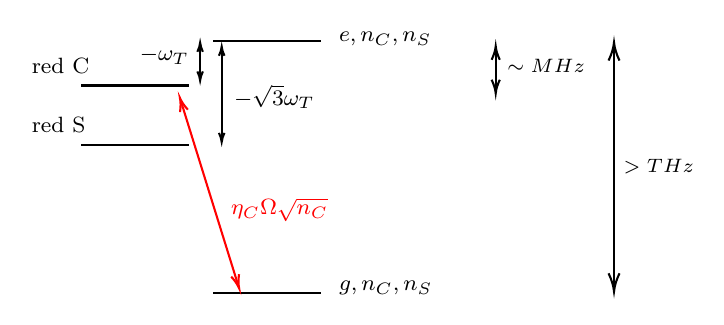
\begin{tikzpicture}[x=0.75pt,y=0.75pt,yscale=-1,xscale=1]
%uncomment if require: \path (0,146); %set diagram left start at 0, and has height of 146

%Straight Lines [id:da8993089849930328] 
\draw    (30.38,59.59) -- (82.31,59.59) ;
%Straight Lines [id:da29699103187525655] 
\draw    (30.38,30.75) -- (82.31,30.75) ;
%Straight Lines [id:da9565575071502495] 
\draw    (93.89,130.93) -- (145.83,130.93) ;
%Straight Lines [id:da38723274535804597] 
\draw    (93.89,9.5) -- (145.83,9.5) ;
%Straight Lines [id:da7230830907382644] 
\draw    (87.59,12.14) -- (87.59,26.36) ;
\draw [shift={(87.59,28.36)}, rotate = 270] [color={rgb, 255:red, 0; green, 0; blue, 0 }  ][line width=0.75]    (4.37,-1.32) .. controls (2.78,-0.56) and (1.32,-0.12) .. (0,0) .. controls (1.32,0.12) and (2.78,0.56) .. (4.37,1.32)   ;
\draw [shift={(87.59,10.14)}, rotate = 90] [color={rgb, 255:red, 0; green, 0; blue, 0 }  ][line width=0.75]    (4.37,-1.32) .. controls (2.78,-0.56) and (1.32,-0.12) .. (0,0) .. controls (1.32,0.12) and (2.78,0.56) .. (4.37,1.32)   ;
%Straight Lines [id:da7613574342882506] 
\draw    (97.98,14.06) -- (97.98,55.96) ;
\draw [shift={(97.98,57.96)}, rotate = 270] [color={rgb, 255:red, 0; green, 0; blue, 0 }  ][line width=0.75]    (4.37,-1.32) .. controls (2.78,-0.56) and (1.32,-0.12) .. (0,0) .. controls (1.32,0.12) and (2.78,0.56) .. (4.37,1.32)   ;
\draw [shift={(97.98,12.06)}, rotate = 90] [color={rgb, 255:red, 0; green, 0; blue, 0 }  ][line width=0.75]    (4.37,-1.32) .. controls (2.78,-0.56) and (1.32,-0.12) .. (0,0) .. controls (1.32,0.12) and (2.78,0.56) .. (4.37,1.32)   ;
%Straight Lines [id:da17453665512381966] 
\draw [color={rgb, 255:red, 255; green, 0; blue, 0 }  ,draw opacity=1 ]   (78.43,38.62) -- (105.81,126.62) ;
\draw [shift={(106.4,128.53)}, rotate = 252.72] [color={rgb, 255:red, 255; green, 0; blue, 0 }  ,draw opacity=1 ][line width=0.75]    (6.56,-1.97) .. controls (4.17,-0.84) and (1.99,-0.18) .. (0,0) .. controls (1.99,0.18) and (4.17,0.84) .. (6.56,1.97)   ;
\draw [shift={(77.84,36.71)}, rotate = 72.72] [color={rgb, 255:red, 255; green, 0; blue, 0 }  ,draw opacity=1 ][line width=0.75]    (6.56,-1.97) .. controls (4.17,-0.84) and (1.99,-0.18) .. (0,0) .. controls (1.99,0.18) and (4.17,0.84) .. (6.56,1.97)   ;
%Straight Lines [id:da35411700829971027] 
\draw    (287,12) -- (287,128) ;
\draw [shift={(287,130)}, rotate = 270] [color={rgb, 255:red, 0; green, 0; blue, 0 }  ][line width=0.75]    (8.74,-2.63) .. controls (5.56,-1.12) and (2.65,-0.24) .. (0,0) .. controls (2.65,0.24) and (5.56,1.12) .. (8.74,2.63)   ;
\draw [shift={(287,10)}, rotate = 90] [color={rgb, 255:red, 0; green, 0; blue, 0 }  ][line width=0.75]    (8.74,-2.63) .. controls (5.56,-1.12) and (2.65,-0.24) .. (0,0) .. controls (2.65,0.24) and (5.56,1.12) .. (8.74,2.63)   ;
%Straight Lines [id:da3640218170366485] 
\draw    (230,13.8) -- (230,32.55) ;
\draw [shift={(230,34.55)}, rotate = 270] [color={rgb, 255:red, 0; green, 0; blue, 0 }  ][line width=0.75]    (6.56,-1.97) .. controls (4.17,-0.84) and (1.99,-0.18) .. (0,0) .. controls (1.99,0.18) and (4.17,0.84) .. (6.56,1.97)   ;
\draw [shift={(230,11.8)}, rotate = 90] [color={rgb, 255:red, 0; green, 0; blue, 0 }  ][line width=0.75]    (6.56,-1.97) .. controls (4.17,-0.84) and (1.99,-0.18) .. (0,0) .. controls (1.99,0.18) and (4.17,0.84) .. (6.56,1.97)   ;

% Text Node
\draw (153,123.4) node [anchor=north west][inner sep=0.75pt]  [font=\footnotesize]  {$\ket{g,n_{C} ,n_{S}}$};
% Text Node
\draw (153,3.4) node [anchor=north west][inner sep=0.75pt]  [font=\footnotesize]  {$\ket{e,n_{C} ,n_{S}}$};
% Text Node
\draw (57,10.9) node [anchor=north west][inner sep=0.75pt]  [font=\footnotesize]  {$-\omega _{T}$};
% Text Node
\draw (102.5,28.9) node [anchor=north west][inner sep=0.75pt]  [font=\footnotesize]  {$-\sqrt{3} \omega _{T}$};
% Text Node
\draw (5,16) node [anchor=north west][inner sep=0.75pt]  [font=\footnotesize] [align=left] {red C};
% Text Node
\draw (5,44.5) node [anchor=north west][inner sep=0.75pt]  [font=\footnotesize] [align=left] {red S};
% Text Node
\draw (290,64.63) node [anchor=north west][inner sep=0.75pt]  [font=\scriptsize]  {$ >THz$};
% Text Node
\draw (234,16.43) node [anchor=north west][inner sep=0.75pt]  [font=\scriptsize]  {$\sim MHz$};
% Text Node
\draw (101,83.63) node [anchor=north west][inner sep=0.75pt]  [font=\footnotesize,color={rgb, 255:red, 255; green, 0; blue, 0 }  ,opacity=1 ]  {$\eta_C \Omega \sqrt{n_{C}}$};


\end{tikzpicture}

\end{center}

\end{tcolorbox}
\vspace{1cm}




\section{Example: Cirac-Zoller CNOT gate}

We want to build a CNOT gate for two qubits. This step is fundamental to get a universal set of operations.\\

\noindent \textbf{Ingredients}:
\begin{itemize}
    \item $2 \times$ 3-level $\{\ket{g}, \ket{e}, \ket{a}\}$ trapped ions (ex: $Ca^+$), where the auxiliary state $\ket{a}$ is not an allowed input.
    \item $2 \times$ focused lasers $L1, L2$ which can be rapidly turned on/off.
    \item $1 \times$ harmonic ion trap.
\end{itemize}
\begin{center}
    

\tikzset{every picture/.style={line width=0.75pt}} %set default line width to 0.75pt        

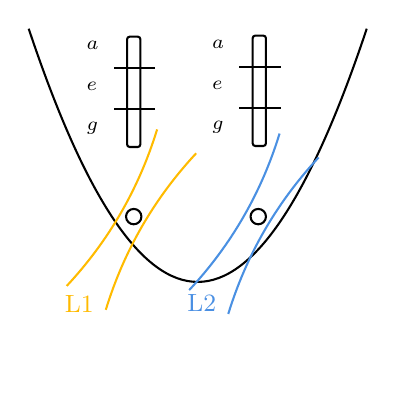
\begin{tikzpicture}[x=0.75pt,y=0.75pt,yscale=-1,xscale=1]
%uncomment if require: \path (0,162); %set diagram left start at 0, and has height of 162

%Shape: Parabola [id:dp6600560249897834] 
\draw   (13.11,11.18) .. controls (67.39,173.84) and (121.68,173.84) .. (175.97,11.18) ;
%Shape: Circle [id:dp18474882329925513] 
\draw   (60,101.7) .. controls (60,99.66) and (61.66,98) .. (63.7,98) .. controls (65.75,98) and (67.41,99.66) .. (67.41,101.7) .. controls (67.41,103.75) and (65.75,105.41) .. (63.7,105.41) .. controls (61.66,105.41) and (60,103.75) .. (60,101.7) -- cycle ;
%Shape: Circle [id:dp1125926223428434] 
\draw   (120,101.7) .. controls (120,99.66) and (121.66,98) .. (123.7,98) .. controls (125.75,98) and (127.41,99.66) .. (127.41,101.7) .. controls (127.41,103.75) and (125.75,105.41) .. (123.7,105.41) .. controls (121.66,105.41) and (120,103.75) .. (120,101.7) -- cycle ;
%Shape: Parabola [id:dp9511655488027904] 
\draw  [color={rgb, 255:red, 255; green, 187; blue, 0 }  ,draw opacity=1 ] (31.42,135.12) .. controls (51.71,113.31) and (66.23,88.17) .. (74.97,59.69) ;
%Shape: Parabola [id:dp36759296152967846] 
\draw  [color={rgb, 255:red, 255; green, 187; blue, 0 }  ,draw opacity=1 ] (93.8,71.19) .. controls (73.51,93.01) and (59,118.15) .. (50.25,146.62) ;
%Shape: Parabola [id:dp36811618670172386] 
\draw  [color={rgb, 255:red, 74; green, 144; blue, 226 }  ,draw opacity=1 ] (90.42,137.12) .. controls (110.71,115.31) and (125.23,90.17) .. (133.97,61.69) ;
%Shape: Parabola [id:dp18893194431896954] 
\draw  [color={rgb, 255:red, 74; green, 144; blue, 226 }  ,draw opacity=1 ] (152.8,73.19) .. controls (132.51,95.01) and (118,120.15) .. (109.25,148.62) ;
%Straight Lines [id:da2309226656139074] 
\draw    (74,30) -- (54,30) ;
%Rounded Rect [id:dp3741809575727877] 
\draw   (60.5,16.28) .. controls (60.5,15.57) and (61.07,15) .. (61.78,15) -- (65.63,15) .. controls (66.33,15) and (66.91,15.57) .. (66.91,16.28) -- (66.91,66.89) .. controls (66.91,67.6) and (66.33,68.18) .. (65.63,68.18) -- (61.78,68.18) .. controls (61.07,68.18) and (60.5,67.6) .. (60.5,66.89) -- cycle ;
%Straight Lines [id:da9684575061600806] 
\draw    (74,50) -- (54,50) ;
%Straight Lines [id:da9880508830624835] 
\draw    (134.5,29.5) -- (114.5,29.5) ;
%Rounded Rect [id:dp6621821890356242] 
\draw   (121,15.78) .. controls (121,15.07) and (121.57,14.5) .. (122.28,14.5) -- (126.13,14.5) .. controls (126.83,14.5) and (127.41,15.07) .. (127.41,15.78) -- (127.41,66.39) .. controls (127.41,67.1) and (126.83,67.68) .. (126.13,67.68) -- (122.28,67.68) .. controls (121.57,67.68) and (121,67.1) .. (121,66.39) -- cycle ;
%Straight Lines [id:da20298612962713958] 
\draw    (134.5,49.5) -- (114.5,49.5) ;

% Text Node
\draw (29,138) node [anchor=north west][inner sep=0.75pt]   [align=left] {{\small \textcolor[rgb]{1,0.73,0}{L1}}};
% Text Node
\draw (88,137.5) node [anchor=north west][inner sep=0.75pt]  [color={rgb, 255:red, 74; green, 144; blue, 226 }  ,opacity=1 ] [align=left] {{\small \textcolor[rgb]{0.29,0.56,0.89}{L2}}};
% Text Node
\draw (39.5,54.9) node [anchor=north west][inner sep=0.75pt]  [font=\scriptsize]  {$\ket{g}$};
% Text Node
\draw (39.5,35.4) node [anchor=north west][inner sep=0.75pt]  [font=\scriptsize]  {$\ket{e}$};
% Text Node
\draw (39.5,15.9) node [anchor=north west][inner sep=0.75pt]  [font=\scriptsize]  {$\ket{a}$};
% Text Node
\draw (100,54.4) node [anchor=north west][inner sep=0.75pt]  [font=\scriptsize]  {$\ket{g}$};
% Text Node
\draw (100,34.9) node [anchor=north west][inner sep=0.75pt]  [font=\scriptsize]  {$\ket{e}$};
% Text Node
\draw (100,15.4) node [anchor=north west][inner sep=0.75pt]  [font=\scriptsize]  {$\ket{a}$};


\end{tikzpicture}

\end{center}

We have seen previously that we need a very good cooling strategy too, since we need $CoM$ phonons at $T\sim0$.

\textbf{Remark}: When a laser is perfectly resonant to a transition, I can go to an interaction picture via a suitable frame change $\tilde{U}$ on the hamiltonian $H$. If
\begin{equation*}
H = \begin{pmatrix}
    \ddots\\
    & \varepsilon_1\\
    &&\varepsilon_2&\Omega\\
    &&\Omega& \varepsilon_2\\
    &&&&\varepsilon_3\\
    &&&&&\ddots\\
\end{pmatrix},
\;\;
\tilde{U} = \begin{pmatrix}
    \ddots\\
    & e^{i\varepsilon_1t}\\
    && e^{i\varepsilon_2t}\\
    &&& e^{i\varepsilon_2t}\\
    &&&& e^{i\varepsilon_3t}\\
    &&&&&\ddots\\
\end{pmatrix}
\end{equation*}
we obtain in the interaction picture as $H_{int} = \tilde{U}H\tilde{U} + i\hbar \dot{\tilde{U}}\tilde{U}^\dag$, i.e.
\begin{equation*}
H_{int} = \begin{pmatrix}
    0\\
    & 0\\
    && 0 & \Omega\\
    && \Omega & 0\\
    &&&& 0\\
    &&&&&0\\
\end{pmatrix}
\end{equation*}
$\Rightarrow$ it is convenient to go to the interaction picture in order to perform calculations, as the bare hamiltonian goes away.




\subsection{Protocol}

The lasers are tuned in the following way:
\begin{itemize}
    \item Laser 1 ($L1$) is focused on ion 1, in resonance to $\ket{g}_1 \leftrightarrow \ket{e}_1$ through a red-sideband transition\\
    $$H_{L1} = \frac{\hbar\eta_C\Omega_1(t)}{2}
    \left( i\ket{e}\bra{g}_1 a_C + h.c. \right)$$
    $$\omega_{L1} \approx \omega_{eg} -\omega_T$$
    \item Laser 2 ($L2$) is focused on ion 2, in resonance to $\ket{g}_2 \leftrightarrow \ket{a}_2$ through a red-sideband transition\\
    $$H_{L2} = \frac{\hbar\eta_C\Omega_2(t)}{2}
    \left( i\ket{a}\bra{g}_2a_C + h.c. \right)$$
    $$\omega_{L2} \approx \omega_{ag} -\omega_T$$
\end{itemize}




\noindent In principle the lasers may show some transient when turned on/off. For this protocol one can take the frequency evolution to be similar to a square function (the laser turns on/off immediately). The protocol consists of the following steps:

\begin{itemize}

% STEP 1
\item \textbf{Step 1} - Laser 2 off, Laser 1 on for $t_1 = \frac{\pi}{\eta_C\Omega_1}$. We call this a $\pi$-PULSE. 
    The unitary operator associated to this operation is
    \begin{align*}
    U_1 &= \exp{ -i\frac{\pi}{\eta_C\Omega_1} \frac{1}{\hbar} H_1 }\\% -i or -1 ??? TODO
    & = \exp{ \frac{ -i \pi}{2}
        \left( i \ket{e}\bra{g}_1a_C - i \ket{g}\bra{e}_1a^\dag_C \right)
    }
    \end{align*}
    and it acts basically as $\sigma_y$ on the states $\ket{g_1, 1}$ and $\ket{e_1, 0}$. 
    Indeed, because of
    $e^{i\alpha\sigma_k} = \cos\alpha \mathds{1} + i \sin\alpha \sigma_k$,
    it is $e^{-i\pi\sigma_y/2} = -i \sigma_y$.
    
    In general, the result of the operation is
    \begin{align*}
        \ket{g_1,0} & \overset{U_1}{\longrightarrow} \;\;\; \ket{g_1, 0}\\
        \ket{e_1, 0} & \longrightarrow
            \;\;\; i\left(\ket{e}\bra{g}_1a - \ket{g}\bra{e}_1a^\dag\right)\ket{e_1, 0} = -i \ket{g_1, 1} 
    \end{align*}
    which is graphically represented as
    \begin{center}
    

\tikzset{every picture/.style={line width=0.75pt}} %set default line width to 0.75pt        

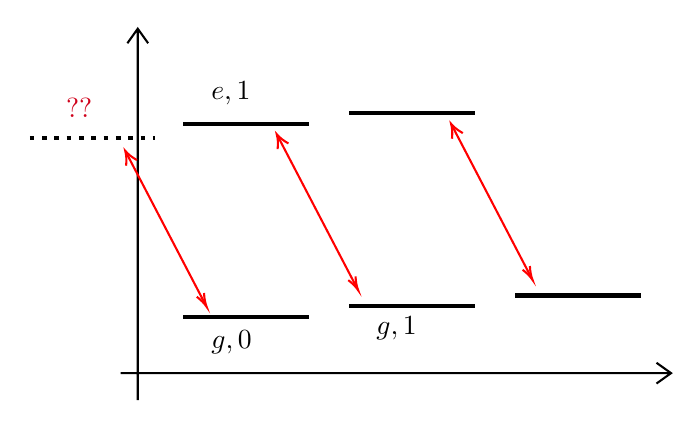
\begin{tikzpicture}[x=0.75pt,y=0.75pt,yscale=-1,xscale=1]
%uncomment if require: \path (0,199); %set diagram left start at 0, and has height of 199

%Shape: Axis 2D [id:dp8238200389598417] 
\draw  (48.83,169.89) -- (313.97,169.89)(57.04,3.94) -- (57.04,182.93) (306.97,164.89) -- (313.97,169.89) -- (306.97,174.89) (52.04,10.94) -- (57.04,3.94) -- (62.04,10.94)  ;
%Straight Lines [id:da9816207475534422] 
\draw [line width=1.5]    (79,143) -- (139.47,143) ;
%Straight Lines [id:da5381598078444266] 
\draw [line width=1.5]    (79,50) -- (139.47,50) ;
%Straight Lines [id:da9628952673311713] 
\draw [line width=1.5]    (159,137.5) -- (219.47,137.5) ;
%Straight Lines [id:da8455519996835935] 
\draw [line width=1.5]    (159,44.5) -- (219.47,44.5) ;
%Straight Lines [id:da8044015159070315] 
\draw [line width=1.5]    (239,132.5) -- (299.47,132.5) ;
%Straight Lines [id:da313266698785474] 
\draw [line width=1.5]  [dash pattern={on 1.69pt off 2.76pt}]  (5,56.5) -- (65.47,56.5) ;
%Straight Lines [id:da6553984074417375] 
\draw [color={rgb, 255:red, 255; green, 0; blue, 0 }  ,draw opacity=1 ]   (124.93,56.54) -- (162.33,128.23) ;
\draw [shift={(163.26,130)}, rotate = 242.44] [color={rgb, 255:red, 255; green, 0; blue, 0 }  ,draw opacity=1 ][line width=0.75]    (6.56,-1.97) .. controls (4.17,-0.84) and (1.99,-0.18) .. (0,0) .. controls (1.99,0.18) and (4.17,0.84) .. (6.56,1.97)   ;
\draw [shift={(124,54.77)}, rotate = 62.44] [color={rgb, 255:red, 255; green, 0; blue, 0 }  ,draw opacity=1 ][line width=0.75]    (6.56,-2.94) .. controls (4.17,-1.38) and (1.99,-0.4) .. (0,0) .. controls (1.99,0.4) and (4.17,1.38) .. (6.56,2.94)   ;
%Straight Lines [id:da14779868058376777] 
\draw [color={rgb, 255:red, 255; green, 0; blue, 0 }  ,draw opacity=1 ]   (51.93,64.54) -- (89.33,136.23) ;
\draw [shift={(90.26,138)}, rotate = 242.44] [color={rgb, 255:red, 255; green, 0; blue, 0 }  ,draw opacity=1 ][line width=0.75]    (6.56,-1.97) .. controls (4.17,-0.84) and (1.99,-0.18) .. (0,0) .. controls (1.99,0.18) and (4.17,0.84) .. (6.56,1.97)   ;
\draw [shift={(51,62.77)}, rotate = 62.44] [color={rgb, 255:red, 255; green, 0; blue, 0 }  ,draw opacity=1 ][line width=0.75]    (6.56,-2.94) .. controls (4.17,-1.38) and (1.99,-0.4) .. (0,0) .. controls (1.99,0.4) and (4.17,1.38) .. (6.56,2.94)   ;
%Straight Lines [id:da6792105316737991] 
\draw [color={rgb, 255:red, 255; green, 0; blue, 0 }  ,draw opacity=1 ]   (208.93,51.54) -- (246.33,123.23) ;
\draw [shift={(247.26,125)}, rotate = 242.44] [color={rgb, 255:red, 255; green, 0; blue, 0 }  ,draw opacity=1 ][line width=0.75]    (6.56,-1.97) .. controls (4.17,-0.84) and (1.99,-0.18) .. (0,0) .. controls (1.99,0.18) and (4.17,0.84) .. (6.56,1.97)   ;
\draw [shift={(208,49.77)}, rotate = 62.44] [color={rgb, 255:red, 255; green, 0; blue, 0 }  ,draw opacity=1 ][line width=0.75]    (6.56,-2.94) .. controls (4.17,-1.38) and (1.99,-0.4) .. (0,0) .. controls (1.99,0.4) and (4.17,1.38) .. (6.56,2.94)   ;

% Text Node
\draw (91,147.9) node [anchor=north west][inner sep=0.75pt]    {$\ket{g,0}$};
% Text Node
\draw (91,27.9) node [anchor=north west][inner sep=0.75pt]    {$\ket{e,1}$};
% Text Node
\draw (170.5,141.4) node [anchor=north west][inner sep=0.75pt]    {$\ket{g,1}$};
% Text Node
\draw (21,36) node [anchor=north west][inner sep=0.75pt]  [color={rgb, 255:red, 208; green, 2; blue, 27 }  ,opacity=1 ] [align=left] {??};


\end{tikzpicture}

    \end{center}

\item \textbf{Step 2} - Laser 1 off, Laser 2 on for $t_2 = \frac{2\pi}{\eta_C\Omega_2}$. We call this a $2\pi$-PULSE.
    The unitary transformation is
    \begin{align*}
    \Rightarrow U_2 &= \exp{ -\frac{i}{\hbar}\frac{2\pi}{\eta_C\Omega_2} H_2 }\\
    & = \exp{ -i\pi \left(
        i\ket{a}\bra{g}_2a_C - 
        i\ket{g}\bra{a}_2a_C^\dag
    \right)
    }
    \end{align*}
    
    The expression acts like $-\mathds{1}$ on the states $\ket{g_2,1}, \ket{a_2, 0}$. Given the possible starting states
    \begin{align*}
        \ket{g_2,0} & \overset{U_2}{\longrightarrow} \;\;\; \ket{g_2, 0}\\
        \ket{e_2, 0} & \longrightarrow \;\;\; \ket{e_2, 0}\\
        \ket{g_2, 1} & \longrightarrow - \ket{g_2, 1}
    \end{align*}
    
    \begin{center}
    

\tikzset{every picture/.style={line width=0.75pt}} %set default line width to 0.75pt        

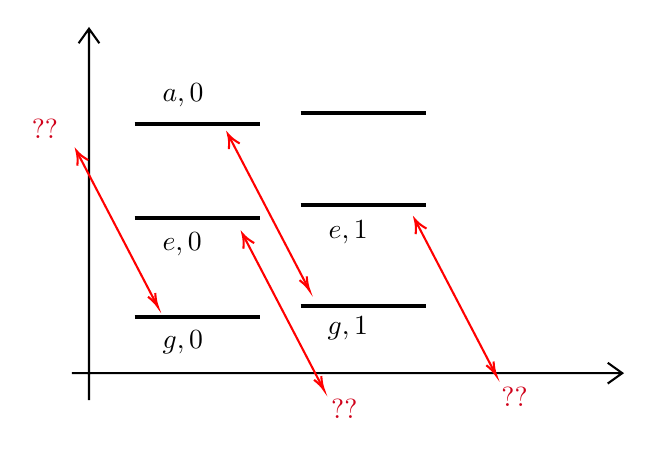
\begin{tikzpicture}[x=0.75pt,y=0.75pt,yscale=-1,xscale=1]
%uncomment if require: \path (0,199); %set diagram left start at 0, and has height of 199

%Shape: Axis 2D [id:dp7044047881463993] 
\draw  (22.83,170.89) -- (287.97,170.89)(31.04,4.94) -- (31.04,183.93) (280.97,165.89) -- (287.97,170.89) -- (280.97,175.89) (26.04,11.94) -- (31.04,4.94) -- (36.04,11.94)  ;
%Straight Lines [id:da8544066902130162] 
\draw [line width=1.5]    (53,144) -- (113.47,144) ;
%Straight Lines [id:da7205922197236949] 
\draw [line width=1.5]    (53,51) -- (113.47,51) ;
%Straight Lines [id:da5372911334007633] 
\draw [line width=1.5]    (133,138.5) -- (193.47,138.5) ;
%Straight Lines [id:da025883166300928573] 
\draw [line width=1.5]    (133,45.5) -- (193.47,45.5) ;
%Straight Lines [id:da8336819480921466] 
\draw [color={rgb, 255:red, 255; green, 0; blue, 0 }  ,draw opacity=1 ]   (98.93,57.54) -- (136.33,129.23) ;
\draw [shift={(137.26,131)}, rotate = 242.44] [color={rgb, 255:red, 255; green, 0; blue, 0 }  ,draw opacity=1 ][line width=0.75]    (6.56,-1.97) .. controls (4.17,-0.84) and (1.99,-0.18) .. (0,0) .. controls (1.99,0.18) and (4.17,0.84) .. (6.56,1.97)   ;
\draw [shift={(98,55.77)}, rotate = 62.44] [color={rgb, 255:red, 255; green, 0; blue, 0 }  ,draw opacity=1 ][line width=0.75]    (6.56,-2.94) .. controls (4.17,-1.38) and (1.99,-0.4) .. (0,0) .. controls (1.99,0.4) and (4.17,1.38) .. (6.56,2.94)   ;
%Straight Lines [id:da8918814843361473] 
\draw [color={rgb, 255:red, 255; green, 0; blue, 0 }  ,draw opacity=1 ]   (25.93,65.54) -- (63.33,137.23) ;
\draw [shift={(64.26,139)}, rotate = 242.44] [color={rgb, 255:red, 255; green, 0; blue, 0 }  ,draw opacity=1 ][line width=0.75]    (6.56,-1.97) .. controls (4.17,-0.84) and (1.99,-0.18) .. (0,0) .. controls (1.99,0.18) and (4.17,0.84) .. (6.56,1.97)   ;
\draw [shift={(25,63.77)}, rotate = 62.44] [color={rgb, 255:red, 255; green, 0; blue, 0 }  ,draw opacity=1 ][line width=0.75]    (6.56,-2.94) .. controls (4.17,-1.38) and (1.99,-0.4) .. (0,0) .. controls (1.99,0.4) and (4.17,1.38) .. (6.56,2.94)   ;
%Straight Lines [id:da2473095698421811] 
\draw [color={rgb, 255:red, 255; green, 0; blue, 0 }  ,draw opacity=1 ]   (188.93,98.54) -- (226.33,170.23) ;
\draw [shift={(227.26,172)}, rotate = 242.44] [color={rgb, 255:red, 255; green, 0; blue, 0 }  ,draw opacity=1 ][line width=0.75]    (6.56,-1.97) .. controls (4.17,-0.84) and (1.99,-0.18) .. (0,0) .. controls (1.99,0.18) and (4.17,0.84) .. (6.56,1.97)   ;
\draw [shift={(188,96.77)}, rotate = 62.44] [color={rgb, 255:red, 255; green, 0; blue, 0 }  ,draw opacity=1 ][line width=0.75]    (6.56,-2.94) .. controls (4.17,-1.38) and (1.99,-0.4) .. (0,0) .. controls (1.99,0.4) and (4.17,1.38) .. (6.56,2.94)   ;
%Straight Lines [id:da5354722999998263] 
\draw [line width=1.5]    (53,96) -- (113.47,96) ;
%Straight Lines [id:da15509678461862553] 
\draw [line width=1.5]    (133,90) -- (193.47,90) ;
%Straight Lines [id:da5426262796400413] 
\draw [color={rgb, 255:red, 255; green, 0; blue, 0 }  ,draw opacity=1 ]   (105.93,105.54) -- (143.33,177.23) ;
\draw [shift={(144.26,179)}, rotate = 242.44] [color={rgb, 255:red, 255; green, 0; blue, 0 }  ,draw opacity=1 ][line width=0.75]    (6.56,-1.97) .. controls (4.17,-0.84) and (1.99,-0.18) .. (0,0) .. controls (1.99,0.18) and (4.17,0.84) .. (6.56,1.97)   ;
\draw [shift={(105,103.77)}, rotate = 62.44] [color={rgb, 255:red, 255; green, 0; blue, 0 }  ,draw opacity=1 ][line width=0.75]    (6.56,-2.94) .. controls (4.17,-1.38) and (1.99,-0.4) .. (0,0) .. controls (1.99,0.4) and (4.17,1.38) .. (6.56,2.94)   ;

% Text Node
\draw (65,148.9) node [anchor=north west][inner sep=0.75pt]    {$\ket{g,0}$};
% Text Node
\draw (145,95.9) node [anchor=north west][inner sep=0.75pt]    {$\ket{e,1}$};
% Text Node
\draw (144.5,142.4) node [anchor=north west][inner sep=0.75pt]    {$\ket{g,1}$};
% Text Node
\draw (2,47) node [anchor=north west][inner sep=0.75pt]  [color={rgb, 255:red, 208; green, 2; blue, 27 }  ,opacity=1 ] [align=left] {??};
% Text Node
\draw (65,101.9) node [anchor=north west][inner sep=0.75pt]    {$\ket{e,0}$};
\draw (65,30) node [anchor=north west][inner sep=0.75pt]    {$\ket{a,0}$};
% Text Node
\draw (146.26,182) node [anchor=north west][inner sep=0.75pt]  [color={rgb, 255:red, 208; green, 2; blue, 27 }  ,opacity=1 ] [align=left] {??};
% Text Node
\draw (228.26,176) node [anchor=north west][inner sep=0.75pt]  [color={rgb, 255:red, 208; green, 2; blue, 27 }  ,opacity=1 ] [align=left] {??};


\end{tikzpicture}

    \end{center}


\item \textbf{Step 3} - Identical to \textit{Step 1}.
    $$\Rightarrow U_3 = U_1$$
    In particular, $U_3\;i\ket{g_1, 1} = + \ket{e_1,0}$.
\end{itemize}


\noindent \textbf{Table of canonical states} - If we consider all the 4 possible inputs, then
\begin{align*}
    \text{Inputs:}\;\;&
    \begin{cases}
        \ket{ g_1, g_2, 0} \\[1pt]
        \ket{ g_1, e_2, 0} \\[1pt]
        \ket{ e_1, g_2, 0} \\[1pt]
        \ket{ e_1, e_2, 0}
    \end{cases}
    \;\; \xrightarrow[L1\;\;\pi]{U_1} \;\;
    \begin{aligned}
        \ket{ g_1, g_2, 0} \\[1pt]
        \ket{ g_1, e_2, 0} \\[1pt]
        - i\ket{ g_1, g_2, 1} \\[1pt]
        - i\ket{ g_1, e_2, 1}
    \end{aligned}
    \;\; \xrightarrow[L2\;\;2\pi]{U_2} \\
    & \xrightarrow{U_2} \;\;
    \begin{aligned}
        \ket{ g_1, g_2, 0} \\[1pt]
        \ket{ g_1, e_2, 0} \\[1pt]
        + i\ket{ g_1, g_2, 1} \\[1pt]
        - i\ket{ g_1, e_2, 1}
    \end{aligned}
    \;\; \xrightarrow[L1\;\;\pi]{U_3=U_1} \qquad
    \text{Outputs:}
    \begin{cases}
        \ket{ g_1, g_2, 0} \\[1pt]
        \ket{ g_1, e_2, 0} \\[1pt]
        \ket{ e_1, g_2, 0} \\[1pt]
        - \ket{ e_1, e_2, 0}
    \end{cases}
\end{align*}

This operation goes from states with zero phonons to other states with zero phonons, but with a switched sign in the fourth input state. Therefore, the protocol acts as a \textbf{control-flip} gate on the second ion (qubit):
\begin{equation*}
    G_{CZ} = U_1 U_2 U_1 = \begin{pmatrix}
        1\\
        &1\\
        &&1\\
        &&&-1
    \end{pmatrix}
    = \begin{quantikz}
        & \ctrl{1} &\qw \\
        & \gate{Z} &\qw \\
    \end{quantikz}
\end{equation*}
from which one can build the CNOT gate as
\begin{center}
$CNOT =\;$
\begin{quantikz}
    & \ctrl{1} &\qw \\
    & \targ{} &\qw \\
\end{quantikz}
$\;\;=\;\;$
\begin{quantikz}
    &\qw      & \ctrl{1} & \qw     &\qw \\
    &\gate{H} & \gate{Z} & \gate{H} &\qw \\
\end{quantikz}
\end{center}

\noindent Being able to create such gate is a fundamental requirement to perform universal quantum computing operations.\\

\noindent \textbf{Note}: The most strict requirement of this protocol is to approach the limit $T=0$ (zero temperature phonon $\sim \mu K$). Some year after Cirac-Zoller\footnote{\href{https://doi.org/10.1103/PhysRevLett.74.4091}{Phys. Rev. Lett. 74, 4091 (1995)} - This is generalized for $N$ ions.} design of a CNOT gate, Klaus Mølmer and Anders Sørensen proposed a solution\footnote{\href{https://doi.org/10.1103/PhysRevLett.82.1971}{Phys. Rev. Lett. 82, 1971 (1999)}} which addressed the strict requirement of the temperature.
